\documentclass[11pt]{article}
\usepackage{../../Utility/Template}
\usepackage{hyperref}
\usepackage{fancyhdr}
\usepackage{lastpage}
\usepackage{caption}

\setcounter{tocdepth}{4}
\setcounter{secnumdepth}{4}

\begin{document}
\newcommand{\Titolo}{\Glossario}

\newcommand{\Redattori}{\SP{} \newline	\ZM{} \newline \RA{} \newline \SH{}}

\newcommand{\Verificatori}{\BM{} \newline \PA{}}

\newcommand{\Approvatore}{\SG{}}

\newcommand{\Distribuzione}{\Proponente{} \newline \VT{} \newline \CR{} \newline Gruppo \Gruppo{}}

\newcommand{\Uso}{Esterno}

\newcommand{\DescrizioneDoc}{Il glossario serve per dare una definizione e chiarire il significato di alcuni termini presenti nella documentazione fornita.}

\newcommand{\pathimg}{../../Utility/images/logo2.png}

\newcommand{\Versionedoc}{1.0.0}
% info generali 

\newcommand{\NomeProgetto}{\textit{HD Viz}}

% fornitore
\newcommand{\Gruppo}{\textit{CodeBusters}}
\newcommand{\Mail}{codebusterswe@gmail.com}

% committenti
\newcommand{\Committente}{\VT \newline \CR}
\newcommand{\VT}{Prof. Vardanega Tullio}
\newcommand{\CR}{Prof. Cardin Riccardo}

% proponenti
\newcommand{\Proponente}{\textit{Zucchetti}}

% codebusters
\newcommand{\SG}{Sassaro Giacomo}
\newcommand{\BM}{Baldisseri Michele}
\newcommand{\ZM}{Zenere Marco}
\newcommand{\PA}{Pirolo Alessandro}
\newcommand{\SP}{Scialpi Paolo}
\newcommand{\SH}{Safdari Hossain}
\newcommand{\RA}{Rago Alessandro}

% ruoli
\newcommand{\Responsabile}{Responsabile di Progetto}
\newcommand{\Amministratore}{Amministratore di Progetto}

% documenti

\newcommand{\SdF}{\textit{Studio di Fattibilità}}
\newcommand{\SdFv}[1]{\textit{Studio di Fattibilità {#1}}}
\newcommand{\PdQ}{\textit{Piano di Qualifica}}
\newcommand{\PdQv}[1]{\textit{Piano di Qualifica {#1}}}
\newcommand{\PdP}{\textit{Piano di Progetto}}
\newcommand{\PdPv}[1]{\textit{Piano di Progetto {#1}}}
\newcommand{\NdP}{\textit{Norme di Progetto}}
\newcommand{\NdPv}[1]{\textit{Norme di Progetto {#1}}}
\newcommand{\AdR}{\textit{Analisi dei Requisiti}}
\newcommand{\AdRv}[1]{\textit{Analisi dei Requisiti {#1}}}
\newcommand{\Glossario}{\textit{Glossario}}
\newcommand{\Glossariov}[1]{\textit{Glossario {#1}}}
\newcommand{\MM}{\textit{Manuale Manutentore}}
\newcommand{\MMv}[1]{\textit{Manuale Manutentore {#1}}}
\newcommand{\MU}{\textit{Manuale Utente}}
\newcommand{\MUv}[1]{\textit{Manuale Utente {#1}}}

% comandi generali
\newcommand{\glo}[1]{#1\ap{G}}
%\newcommand{\glo}[1]{\textsc{#1\textsuperscript{\textit{G}}}}

\setlength{\parindent}{-0.1em}
\frontespizio
\fancydoc
\newpage	
\section*{Registro delle modifiche}
{
\rowcolors{2}{colorePanna}{coloreGrigietto}
\renewcommand{\arraystretch}{1.5}
\centering
\begin{longtable}{c C{2.6cm} C{3cm} C{3cm} C{5cm}}
\rowcolor{coloreRosso}
\textcolor{white}{\textbf{Versione}}&
\textcolor{white}{\textbf{Data}}&
\textcolor{white}{\textbf{Nominativo}}&
\textcolor{white}{\textbf{Ruolo}}&
\textcolor{white}{\textbf{Descrizione}}\\	
\endhead

1.0.0 & 08/01/2021 & \SG{} & Responsabile & Approvazione del documento \\

0.3.0 & 04/01/2021 & \SH{} & Verificatore & Revisione complessiva del documento \\

0.2.6 & 22/12/2020 & \BM{} & Responsabile & Stesura \S A e \S B \\

0.2.5 & 21/12/2020 & \BM{} & Responsabile & Stesura \S 6\\

0.2.4 & 21/12/2020 & \SG{} & Responsabile & Aggiunti grafici \\

0.2.3 & 21/12/2020 & \BM{} & Responsabile & Stesura \S 5.3 e \S 5.4\\

0.2.2 & 20/12/2020 & \SG{} & Responsabile & Fine stesura \S 5.2 e stesura \S 5.5 \\

0.2.1 & 20/12/2020 & \BM{} & Responsabile & Stesura \S 5.3 e \S 5.4\\

0.2.0 & 19/12/2020 & \ZM{} & Verificatore & Revisione complessiva del documento \\

0.1.6 & 19/12/2020 & \SG{} & Responsabile & Inizio stesura \S 5 \\

0.1.5 & 18/12/2020 & \PA{} & Amministratore & Fine stesura \S 4.3\\

0.1.4 & 18/12/2020 & \SG{} & Responsabile & Stesura \S 4.4 \\

0.1.3 & 17/12/2020 & \BM{} & Responsabile & Stesura \S 4.2 e iniziata \S 4.3 \\

0.1.2 & 17/12/2020 & \SG{} & Responsabile & Stesura \S 4.1 \\

0.1.1 & 17/12/2020 & \SG{},\newline \BM{} & Responsabili & Stesura \S 3.2 \\

0.1.0 & 17/12/2020 & \ZM{} & Verificatore & Revisione complessiva del documento \\

0.0.5 & 16/12/2020 & \BM{} & Responsabile & Stesura \S 2.2 e \S 2.3 \\
		
0.0.4 & 15/12/2020 & \PA{} & Amministratore & Inizio stesura \S 2 \\

0.0.3 & 15/12/2020 & \SG{} & Responsabile & Stesura \S 3.1 \\

0.0.2 & 14/12/2020 & \PA{} & Amministratore & Aggiunta \S 1 \\

0.0.1 & 14/12/2020 & \SG{} & Responsabile & Creata struttura del documento Latex \\
		
\end{longtable}
}

\newpage
\tableofcontents
\newpage
\listoftables
\newpage
\listoffigures
\newpage
\section{Introduzione}
\subsection{Scopo del documento}
Questo documento ha lo scopo di fornire tutte le informazioni relative al sistema di controllo di qualità per i processi ed i prodotti, basandosi su assunti misurabili ma adattati alle esigenze del proprio progetto.
Esso deve implementare degli standard che permettano il miglioramento continuo, tracciando periodicamente tramite misurazioni i risultati ottenuti sfruttandoli per definire azioni migliorative. All'interno del \textit{Piano di Qualifica} vengono anche raccolte le definizioni dei test, il loro stato e il loro tracciamento. 

\subsection{Scopo del capitolato}
Oggigiorno, anche i programmi più tradizionali gestiscono e memorizzano una grande mole di dati; di conseguenza servono software in grado di eseguire un'analisi e un'interpretazione delle informazioni.\\
Il \glo{capitolato} C4 ha come obiettivo quello di creare un'applicazione di visualizzazione di dati con numerose dimensioni in modo da renderle comprensibili all'occhio umano.  Lo scopo del prodotto sarà quello di fornire all'utente diversi tipi di visualizzazioni e di algoritmi per la riduzione dimensionale in modo che, attraverso un processo esplorativo, l'utilizzatore del prodotto possa studiare tali dati ed evidenziarne degli eventuali \glo{cluster}. 

\subsection{Glossario}
Per evitare ambiguità relative alle terminologie utilizzate, è stato compilato il \Glossariov{2.0.0}. In questo documento sono riportati tutti i termini importanti e con un significato particolare. Questi termini sono evidenziati da una 'G' ad apice.

\subsection{Riferimenti}
\subsubsection{Riferimenti normativi}
\begin{itemize}	
\item \textbf{\NdPv{v 2.0.0}};
	
\item \textbf{Capitolato d'appalto C4 - HD Viz: visualizzazione di dati multidimensionali}:\\
	\textcolor{blue}{\url{https://www.math.unipd.it/~tullio/IS-1/2020/Progetto/C4.pdf}}

\end{itemize}

\subsubsection{Riferimenti informativi}
\begin{itemize}
	\item \textbf{Software Engineering - Ian Sommerville - 10 th Edition}: \\
	Parte 4 - Software Management
	\begin{itemize}
	\item Capitolo 24 - Quality Management:
		\begin{itemize}
			\item Paragrafo 24.1 - Software Quality (da pag. 703 a 705);
			\item Paragrafo 24.3 - Reviews and inspection (da pag. 710 a 714);
			\item Paragrafo 24.5 - Software measurement (da pag. 717 a 725).
		\end{itemize}
	\end{itemize}
	
	\item \textbf{Slide T12 del corso Ingegneria del Software - Qualità di prodotto}:\\
	\textcolor{blue}{\url{https://www.math.unipd.it/~tullio/IS-1/2020/Dispense/L12.pdf}}
	\begin{itemize}
		\item Slide 8 - I 7 principi del Sistema Qualità;
		\item Slide 12,13 - Cosa significa qualità SW;
		\item Slide 17 - Il processo di valutazione.
	\end{itemize}
	
	\item \textbf{Slide T13 del corso Ingegneria del Software - Qualità di processo}:\\
	\textcolor{blue}{\url{https://www.math.unipd.it/~tullio/IS-1/2020/Dispense/L13.pdf}}
		\begin{itemize}
		\item Slide 3 - Modello concettuale di processo;
		\item Slide 11 - I 5 livelli di maturità;
		\item Slide 23 - Riepilogo: la ricerca della qualità.
	\end{itemize}
	
	\item \textbf{Slide T14 del corso Ingegneria del Software - Verifica e validazione}:\\
	\textcolor{blue}{\url{https://www.math.unipd.it/~tullio/IS-1/2020/Dispense/L14.pdf}}
	\begin{itemize}
		\item Slide 6 - Verifica e validazione nello sviluppo; 
		\item Slide 15 - Analisi dinamica: tipi di test.
	\end{itemize}
	
	\item \textbf{Indice di Gulpease}:\\
	\textcolor{blue}{\url{https://it.wikipedia.org/wiki/Indice_Gulpease}}
	
	\item \textbf{Averege Cyclomatic complexity}:\\
	\textcolor{blue}{\url{https://eslint.org/docs/rules/complexity}}
	
\end{itemize}
\newpage
\section{Analisi dei rischi}
Durante lo svolgimento di un progetto di una certa complessità bisogna fare molta attenzione ai possibili rischi a cui il gruppo può andare in contro. Questi possono avere conseguenze particolarmente negative sul lavoro e sul rispetto delle scadenze e risulta quindi necessaria un'attenta analisi, volta alla loro mitigazione.\\Questa attività richiede attenzione costante e ha l'obbiettivo di fare delle previsioni sui problemi che si potrebbero verificare durante tutto il percorso, classificandoli in base alla loro entità e apportando delle risoluzioni.\\
Di seguito è riportata una tabella che riassume tutte le informazioni, realizzata con le seguenti fasi:
\begin{itemize}
\item \textbf{Identificazione:} attività che permette d'individuare gli eventi che potrebbero causare problemi durante l'avanzamento del progetto;
\item \textbf{Analisi:} studio degli eventi rilevati ed assegnazione di un indice di gravità e di una probabilità di occorrenza, rilevando così l'impatto che avrebbero nel progetto;
\item \textbf{Controllo:} pianificazione di una metodologia per evitare che
si verifichino i rischi individuati, stabilendo come agire nel caso in cui questi si riscontrassero;
\item \textbf{Monitoraggio:} durante lo svolgimento del progetto viene costantemente eseguito un controllo per:
	\begin{itemize}
		\item rilevare eventuali nuovi indicatori di rischio;
		\item aggiornare le informazioni già presenti.
	\end{itemize}
Questo fase risulta essere fondamentale perché con il tempo gli effetti sui rischi possono variare ed è necessario riportarli periodicamente all'attenzione di tutto il gruppo.
\end{itemize}

\subsection{Categorie}
I rischi sono stati suddivisi nelle seguenti categorie:
\begin{itemize}
\item \textbf{Tecnologie scelte: T}
\item \textbf{Rapporti interpersonali: I}
\item \textbf{Organizzazione del lavoro: O}
\end{itemize}
I rischi sono identificati dal seguente codice:
\begin{center}
	\textbf{R\{Iniziale categoria\}\{Numero progressivo\}}
\end{center}
\subsubsection{Rischi relativi alle tecnologie}
\rowcolors{1}{coloreGrigietto}{colorePanna}
\begin{center}
Tabella 2.1: Tabella dei rischi tecnologici
\end{center}

\renewcommand{\arraystretch}{1.5}
\renewcommand\extrarowheight{1.5pt}
\begin{longtable}{C{2cm} C{5cm} C{5cm} C{3cm}}
		\rowcolor{coloreRosso}
		\textcolor{white}{\textbf{Codice}} & 
		\textcolor{white}{\textbf{Descrizione}} & 
		\textcolor{white}{\textbf{Identificazione}} & 
		\textcolor{white}{\textbf{Grado}} \\
		\endfirsthead
	    \rowcolor{white}\multicolumn{4}{c}{\textit{Continua nella pagina successiva...}}\\
	    \endfoot
	    \endlastfoot

%--------------------------------------------
\textbf{RT1} \newline Scarsa esperienza &

Tutti i membri del gruppo non hanno ancora un'esperienza tale da affrontare un progetto di questa complessità senza l'insorgere di problemi operativi. & 

Ciascun membro del gruppo deve comunicare con assoluta trasparenza eventuali difficoltà incontrate. Il \textit{Responsabile} ha il compito di rilevare le varie lacune e favorire la condivisione delle conoscenze tra i componenti del team.  & 

\parbox{2.2cm}{
\begin{center}
Pericolosità: \textbf{Elevata} \newline Occorrenza: \textbf{Elevata} 
\end{center} } \\

\multicolumn{4}{c}{\parbox{16cm}{\textbf{Piano di contingenza:} I compiti con difficoltà maggiore verranno assegnati a più componenti, in modo da favorire l'assistenza reciproca.} } \\

%--------------------------------------------
\textbf{RT2} \newline Tecnologie da usare &

La documentazione disponibile per l'utilizzo delle tecnologie interessate è molto approfondita. Il tempo di apprendimento potrebbe causare dei ritardi nello svolgimento dei lavori. & 

Il \textit{Responsabile} ha il compito di monitorare la preparazione dei membri rispetto ai compiti assegnati.  & 

\parbox{2.2cm}{
\begin{center}
Pericolosità: \textbf{Elevata} \newline Occorrenza: \textbf{Media} 
\end{center} } \\

\multicolumn{4}{c}{\parbox{16cm}{\textbf{Piano di contingenza:} In casi di particolare difficoltà è prevista una ridistribuzione del carico di lavoro.} } \\

%--------------------------------------------
\textbf{RT3} \newline Strumenti software &

Il team si affida a strumenti software di terze parti e piattaforme online. Potrebbe esserci il rischio di perdita di dati o non operatività. & 

Qualsiasi membro ha il compito di avvisare il \textit{Responsabile} e gli altri componenti in caso di rilevamento di problemi.  & 

\parbox{2.2cm}{
\begin{center}
Pericolosità: \textbf{Media-Elevata} \newline Occorrenza: \textbf{Bassa} 
\end{center} } \\

\multicolumn{4}{c}{\parbox{16cm}{\textbf{Piano di contingenza:} effettuare un backup dei dati periodico su altre piattaforme.} } \\


%--------------------------------------------
\textbf{RT4} \newline Problemi hardware &

Tutti i componenti del gruppo utilizzano dispositivi personali per lavorare al progetto. Guasti hardware potrebbero causare notevoli disagi e perdite di tempo. & 

Ciascun membro dovrà, nei limiti del possibile, evitarli ed avvisare il \textit{Responsabile} e gli altri componenti i problemi riscontrati.  & 

\parbox{2.2cm}{
\begin{center}
Pericolosità: \textbf{Media} \newline Occorrenza: \textbf{Bassa} 
\end{center} } \\

\multicolumn{4}{c}{\parbox{16cm}{\textbf{Piano di contingenza:} ogni componente deve rispettare l'utilizzo degli strumenti stabiliti nelle \textit{Norme di progetto} per evitare perdite di dati.} } \\
\end{longtable}

\subsubsection{Rischi relativi ai rapporti interpersonali}

\begin{center}
Tabella 2.2: Tabella dei rischi interpersonali
\end{center}
\rowcolors{1}{coloreGrigietto}{colorePanna}
\begin{longtable}{C{2cm} C{5cm} C{5cm} C{3cm}}
		\rowcolor{coloreRosso}
		\textcolor{white}{\textbf{Codice}} & 
		\textcolor{white}{\textbf{Descrizione}} & 
		\textcolor{white}{\textbf{Identificazione}} & 
		\textcolor{white}{\textbf{Grado}} \\
		\endfirsthead
	    \rowcolor{white}\multicolumn{4}{c}{\textit{Continua nella pagina successiva...}}\\
	    \endfoot
	    \endlastfoot

%--------------------------------------------
\textbf{RI1} \newline Collaborazione a distanza &

A causa della situazione di emergenza sanitaria dovuta al virus \textit{Covid-19}, il gruppo potrebbe trovarsi in difficoltà a lavorare e a comunicare sia internamente che con il \textit{proponente}, causando pesanti conseguenze nello svolgimento del progetto. & 

Ciascun membro del gruppo deve utilizzare le piattaforme stabilite e mantenere una comunicazione attiva. Inoltre dovrà adattarsi alle politiche interne dell'azienda proponente per garantire la collaborazione.  & 

\parbox{2.2cm}{
\begin{center}
Pericolosità: \textbf{Elevata} \newline Occorrenza: \textbf{Media} 
\end{center} } \\

\multicolumn{4}{c}{\parbox{16cm}{\textbf{Piano di contingenza:} il gruppo ha predisposto molteplici canali di comunicazione su dispositivi fissi e mobili. Inoltre si devono effettuare riunioni frequenti sia internamente che con il \textit{proponente}.} } \\

%--------------------------------------------
\textbf{RI2} \newline Conflitti decisionali &

Alcuni componenti potrebbero essere in disaccordo rispetto ad alcune decisioni, provocando l'insorgere di conflitti e situazioni spiacevoli. & 

Ciascun membro del gruppo deve esporre con assoluta trasparenza le proprie opinioni, mentre il \textit{Responsabile} dovrà favorire una buona collaborazione.  & 

\parbox{2.2cm}{
\begin{center}
Pericolosità: \textbf{Media} \newline Occorrenza: \textbf{Media} 
\end{center} } \\

\multicolumn{4}{c}{\parbox{16cm}{\textbf{Piano di contingenza:} tutte le proposte devono essere valutate e discusse, con l'unico obbiettivo di scegliere quelle più adatte al bene del progetto.} } \\

%--------------------------------------------
\textbf{RI3} \newline Comunicazione interna &

In alcuni momenti i membri del team potrebbero non essere reperibili, causando dei ritardi nello svolgimento delle riunioni prefissate. & 

Ciascun componente deve comunicare con dovuto anticipo eventuali momenti di irreperibilità attraverso i canali utilizzati dal gruppo di lavoro.  & 

\parbox{2.2cm}{
\begin{center}
Pericolosità: \textbf{Media} \newline Occorrenza: \textbf{Bassa} 
\end{center} } \\

\multicolumn{4}{c}{\parbox{16cm}{\textbf{Piano di contingenza:} il gruppo ha organizzato degli incontri a cadenza fissa in modo da essere sempre allineati con l'avanzamento del progetto.} } \\

%--------------------------------------------
\textbf{RI4} \newline Comunicazione esterna &

Il gruppo potrebbe avere una scarsa comunicazione con il \textit{proponente}, instaurando un cattivo rapporto di collaborazione e causando rallentamenti con l'avanzamento del progetto. & 

Sia il \textit{proponente} che il gruppo devono comunicare eventuali difficoltà che non permettano una normale comunicazione, cercando di trovare dei metodi alternativi a quelli prefissati per mantenerla attiva.  & 

\parbox{2.2cm}{
\begin{center}
Pericolosità: \textbf{Media} \newline Occorrenza: \textbf{Bassa} 
\end{center} } \\

\multicolumn{4}{c}{\parbox{16cm}{\textbf{Piano di contingenza:} esporre periodicamente quesiti e dubbi al \textit{proponente}, effettuando delle riunioni e mostrando l'avanzamento del progetto.} } \\

%--------------------------------------------
\textbf{RI5} \newline Contrasti &

Come in qualsiasi attività collaborative con più persone potrebbero crearsi dei conflitti di varia entità e natura. & 

Tutti i componenti devono limitare le tensioni ed evitare che queste influiscano sull'avanzamento del progetto.  & 

\parbox{2.2cm}{
\begin{center}
Pericolosità: \textbf{Media} \newline Occorrenza: \textbf{Bassa} 
\end{center} } \\

\multicolumn{4}{c}{\parbox{16cm}{\textbf{Piano di contingenza:} tutti i membri non interessati nella controversia, insieme al \textit{Responsabile}, hanno il compito di sedare i contrasti che si possono instaurare durante tutto il periodo.} } \\
\end{longtable}

\subsubsection{Rischi relativi all'organizzazione}

\begin{center}
Tabella 2.3: Tabella dei rischi organizzativi
\end{center}
\rowcolors{1}{coloreGrigietto}{colorePanna}
\begin{longtable}{C{2cm} C{5cm} C{5cm} C{3cm}}
		\rowcolor{coloreRosso}
		\textcolor{white}{\textbf{Codice}} & 
		\textcolor{white}{\textbf{Descrizione}} & 
		\textcolor{white}{\textbf{Identificazione}} & 
		\textcolor{white}{\textbf{Grado}} \\
		\endfirsthead
	    \rowcolor{white}\multicolumn{4}{c}{\textit{Continua nella pagina successiva...}}\\
	    \endfoot
	    \endlastfoot

%--------------------------------------------
\textbf{RO1} \newline Calcolo delle tempistiche &

L'inesperienza e la complessità del progetto potrebbero portare al non rispetto delle scadenze e a continue modifiche nel calcolo del consumo delle risorse. & 

A ciascuno componente saranno affidati dei compiti. Sarà onere a chi appartiene il compito comunicare tutte le difficoltà riscontrate ed eventuali ritardi nel rispetto delle scadenze.  & 

\parbox{2.2cm}{
\begin{center}
Pericolosità: \textbf{Elevata} \newline Occorrenza: \textbf{Media} 
\end{center} } \\

\multicolumn{4}{c}{\parbox{16cm}{\textbf{Piano di contingenza:} in caso di problematiche il \textit{Responsabile} ha il compito di assegnare nuove risorse per concludere l'attività. Inoltre tutti i membri devono collaborare per evitare situazioni di questa tipologia.} } \\

%--------------------------------------------
\textbf{RO2} \newline Costi &

La pianificazione prevede un costo per ogni attività. Essendo il gruppo inesperto potrebbero essere presi in considerazioni dei valori poco veritieri.  & 

Ciascun componente del gruppo ha il compito di prendere nota delle proprie ore dedicato allo studio personale e al lavoro.  & 

\parbox{2.2cm}{
\begin{center}
Pericolosità: \textbf{Elevata} \newline Occorrenza: \textbf{Media} 
\end{center} } \\

\multicolumn{4}{c}{\parbox{16cm}{\textbf{Piano di contingenza:} monitorare la quantità di lavoro svolta da ciascun componente ed aggiornare i valori per tutto l'avanzamento del progetto. In caso di variazioni consistenti è necessario comunicarle al \textit{proponente}. } } \\

%--------------------------------------------
\textbf{RO3} \newline Impegni &

Tutti i membri del gruppo potrebbero causare problemi all'avanzamento del progetto per impegni sia accademici che personali.  & 

Ciascun componente ha il dovere di comunicare al gruppo tutti gli impegni, in modo da favorire un'organizzazione ottimale delle varie attività.  & 

\parbox{2.2cm}{
\begin{center}
Pericolosità: \textbf{Bassa} \newline Occorrenza: \textbf{Media} 
\end{center} } \\

\multicolumn{4}{c}{\parbox{16cm}{\textbf{Piano di contingenza:} utilizzare un calendario condiviso e visibile a tutto il gruppo, in modo da assegnare correttamente incarichi e scadenze. } } \\

%--------------------------------------------
\textbf{RO3} \newline Modifiche dei requisiti &

Durante lo sviluppo del prodotto software, l'azienda potrebbe decidere di modificare i requisiti obbligatori, causando problemi interni sull'organizzazione delle attività e scadenze che erano state prefissate.  & 

Il gruppo deve mantenere una comunicazione attiva e un rapporto collaborativo con il \textit{proponente}, in modo da percepire le intenzioni rispetto al prodotto finale.  & 

\parbox{2.2cm}{
\begin{center}
Pericolosità: \textbf{Elevata} \newline Occorrenza: \textbf{Bassa} 
\end{center} } \\

\multicolumn{4}{c}{\parbox{16cm}{\textbf{Piano di contingenza:} fare riferimento alle precauzioni stabilite per \textbf{RI4}. } } \\

\end{longtable}
\newpage
\section{Modello di sviluppo}
Il gruppo ha deciso di utilizzare il modello incrementale.
\subsection{Modello incrementale}
Il modello incrementale prevede rilasci multipli e successivi, ciascuno di questi realizza un incremento di funzionalità.
É richiesta dunque una classificazione preliminare dei requisiti atta ad individuare i più importanti, i quali devono essere sviluppati nei primi incrementi, così da avere fin da subito un prodotto funzionante, che verrà via via integrato.
L'adozione di questo modello comporta i seguenti vantaggi:
\begin{itemize}
\item Le funzionalità primarie hanno priorità nello sviluppo, così facendo queste vengono verificate più volte;
\item L'avere un prodotto funzionante già dai primi incrementi permette subito al proponente di valutarne le funzioni primarie;
\item Ogni incremento riduce il rischio di fallimento, con un approccio predisposto ai cambiamenti;
\item L'analisi dei requisiti può essere raffinata tramite la progettazione di dettaglio ad ogni incremento;
\item Le modifiche e la correzione degli errori sono più economiche;
\item Le fasi di verifica e test sono facilitate perché mirate a un singolo incremento.
\end{itemize}
\subsection{Incrementi individuati}
In seguito è riportata la tabella con indicati gli incrementi individuati durante la fase di analisi con il rispettivo obiettivo e i requisiti ad esso associati.
I requisiti riportati nella tabella includono tutti i requisiti figli. Tutti i requisiti non riportati sono da intendersi soddisfatti, in parte, da ogni incremento.
Ogni requisito è individuato dal suo codice identificativo, reperibile nel documento \AdRv{}.

\rowcolors{1}{coloreGrigietto}{colorePanna}
\begin{longtable}{C{3cm} C{7cm} C{2cm} C{2cm}}
\rowcolor{coloreRosso}
\textcolor{white}{\textbf{Incremento}} & 
\textcolor{white}{\textbf{Obiettivo dell'incremento}} & 
\textcolor{white}{\textbf{Requisiti}} &
\textcolor{white}{\textbf{Casi d'uso}}\\
\endfirsthead
\rowcolor{white}\multicolumn{4}{c}{\textit{Continua nella pagina successiva...}}\\
\endfoot
\rowcolor{white}\caption{Tabella degli incrementi}
\endlastfoot

%------------------------------------------
Incremento 0 & 
Caricamento dati tramite file e selezione delle dimensioni da utilizzare & 
R1F1 \newline R1F3 & 
UC1.1 \newline UC2\\
%-----------------------------------------
Incremento 1 &
Visualizzazione \glo{Scatter Plot Matrix} & 
R1F5.1 & 
UC3.1 \\
%------------------------------------------
Incremento 2 & 
Personalizzazione della visualizzazione Scatter Plot Matrix & 
R3F10 \newline R3F11 & 
UC4.1\\
%------------------------------------------
Incremento 3 & 
Visualizzazione \glo{Heat Map} e relativa personalizzazione & 
R1F5.2 \newline R1F5.2.1 \newline R3F10 \newline R3F11 & 
UC3.2 \newline UC4.2\\
%------------------------------------------
Incremento 4 & 
Visualizzazione \glo{Force Field} e relativa personalizzazione & 
R1F5.3 \newline R3F10 \newline R3F11 & 
UC3.3 \newline UC4.3\\
%------------------------------------------
Incremento 5 & 
Visualizzazione \glo{Proiezione Lineare Multi Asse} e relativa personalizzazione & 
R1F5.4 \newline R3F10 \newline R3F11& 
UC3.4 \newline UC4.4\\
%------------------------------------------
Incremento 6 & 
Gestione della sessione & 
R2F4 & 
UC5 \newline UC6\\
%------------------------------------------
Incremento 7 & 
Implementazione di un \glo{database} per il caricamento dati attraverso \glo{query} & 
R1F1.2 & 
UC1.2\\
%------------------------------------------
Incremento 8 & 
Perfezionamento del codice con correzioni ricevute durante la \textit{Technology Baseline} e dal proponente & 
Non saranno aggiunte nuove funzionalità software & 
Non saranno aggiunte nuove funzionalità software\\

\end{longtable}

\newpage
\section{Pianificazione}
La pianificazione di progetto viene suddivisa nelle seguenti fasi:
\begin{enumerate}

	\item \textbf{Analisi};
	\item \textbf{Progettazione della \textit{technology baseline}};
	\item \textbf{Codifica del \textit{proof of concept}};
	\item \textbf{Progettazione di dettaglio e codifica};
	\item \textbf{Completamento e raffinamento delle funzionalità};
	\item \textbf{Validazione e collaudo}.
\end{enumerate}

Le fasi \textit{(3), (4)} e \textit{(5)} sono di supporto al gruppo in modo da rispettare le scadenze per lo sviluppo del progetto (riportate a \S 1.4.3). La presenza di tali fasi ha lo scopo di aumentare la comprensione del documento e non deve essere considerata per la scansione degli incrementi, in modo da non collidere con la natura del modello di sviluppo scelto. Per questo motivo non sono citate in \S 5 e \S 6.
\subsection{Analisi}
Questa fase comincia con la presentazione dei capitolati d'appalto e termina con la data di consegna per la \textit{Revisione dei Requisiti}, ovvero dal 05-11-2020 al 11-01-2021.
In questo periodo verranno redatti tutti i documenti necessari e verrà fatta un'analisi approfondita del capitolato scelto dal gruppo \Gruppo{}.

\subsubsection{Obiettivi}
Organizzazione interna del team e stesura di tutti i documenti.

\subsubsection{Periodi e attività}
La pianificazione di questa fase è stata organizzata nei seguenti periodi:
\begin{itemize}
\item \textit{Dal 05-11-2020 al 04-12-2020}: individuazione degli strumenti per la comunicazione interna e discussione dei capitolati proposti. Inizio della stesura dello \SdF{} con \glo{milestone} il 10-12-2020;

\item \textit{Dal 05-12-2020 al 22-12-2020}: stesura delle \NdP{} e del \PdP{} e iniziata inoltre la stesura dell'\AdR{}. Il 22-12-2020 il gruppo ha fissato una milestone\glo{} per la verifica dei prodotti;

\item \textit{Dal 23-12-2020 al 05-01-2021}: il gruppo si dedica all'\AdR{} e al contempo inizia la stesura del \PdQ{}. Il 05-01-2020 il gruppo fissa un'ulteriore milestone\glo{} per verificare che tutti i documenti siano stati completati correttamente;

\item \textit{Dal 06-01-2021 al 11-01-2021}: si svolge attività di verifica su tutti i documenti, si completano eventualmente documenti in ritardo. Si uniformano tutti i documenti stando alle regole stabilite nelle \NdP{}.
\end{itemize}

\begin{landscape}

\begin{figure}[h]
	\centering
	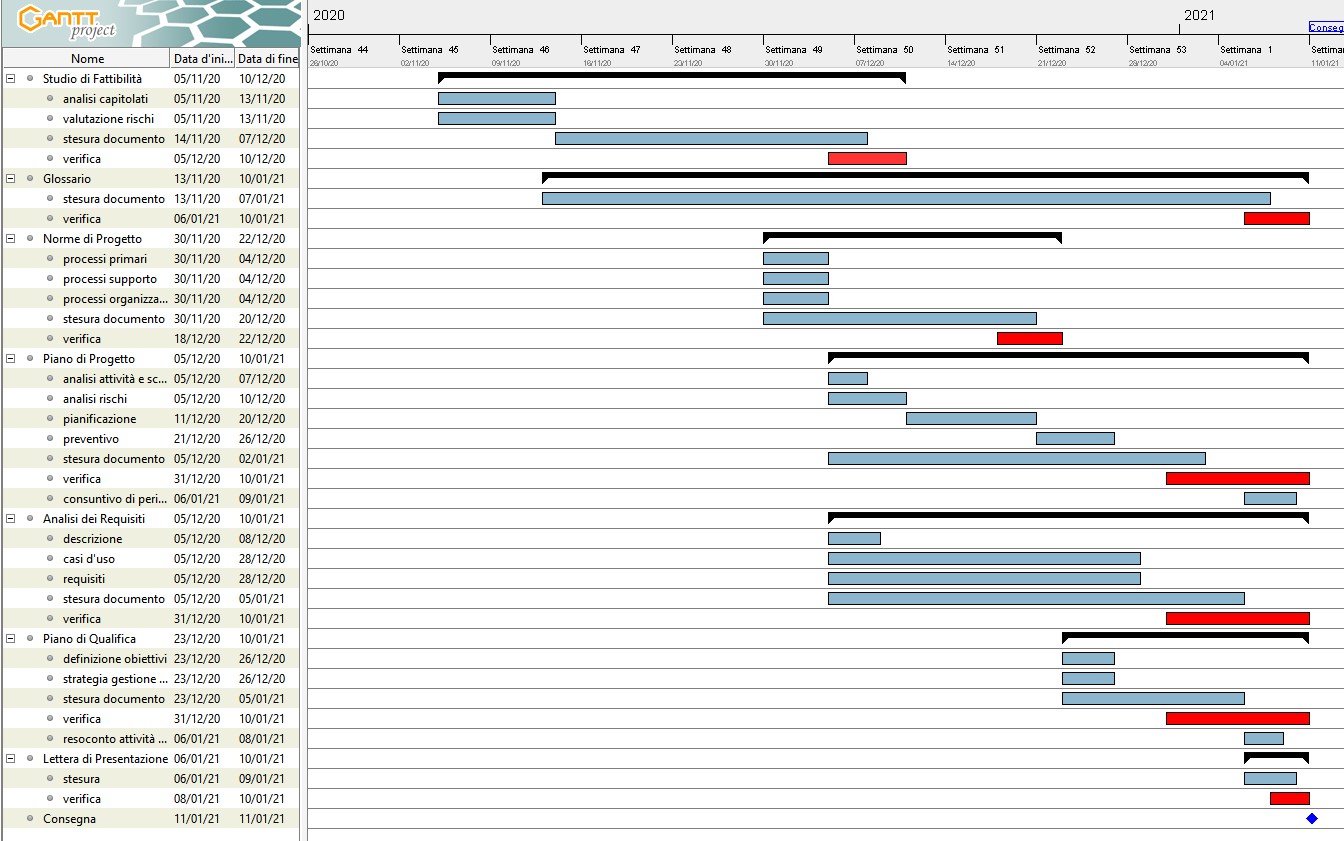
\includegraphics[width=\linewidth]{Images/GanttPianificazioneAnalisi.PNG}
	\caption{Diagramma di Gantt dell'attività di analisi}
\end{figure}

\end{landscape}




\newpage
\subsection{Progettazione della Technology Baseline}
A causa della concomitanza con la sessione accademica, il team ha fissato la prima \glo{milestone} al termine di questo periodo. 
\subsubsection{Obiettivi}
Il gruppo dovrà aver iniziato lo studio delle tecnologie per la \textit{Technology Baseline}, oltre ad aver controllato buona parte della documentazione.
\subsubsection{Periodi e attività}
Questo periodo è unico e ha inizio il giorno 18-01-2021, successivamente alla revisione dei requisiti, con termine fissato per il giorno 07-02-2021. Comprende attività di: 
\begin{itemize}
\item \textbf{Incremento e verifica dei documenti}: se fosse necessario, i documenti prodotti dal team verranno integrati;
\item \glo{\textbf{Technology Baseline}}: viene fatta un'analisi ad alto livello per comprendere le tecnologie coinvolte.
\end{itemize}

\begin{figure}[h]
	\centering	
	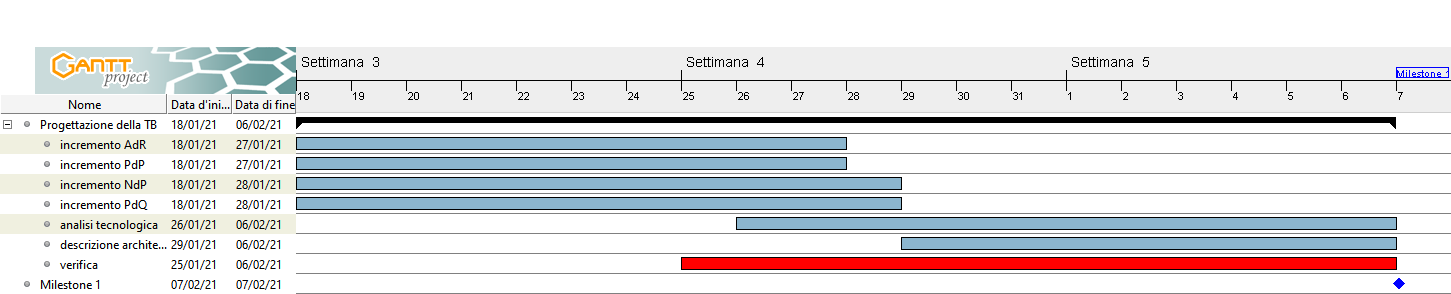
\includegraphics[width=\linewidth]{Images/GanttPianificazioneProgettazioneTB.PNG}
	\caption{Diagramma di Gantt dell'attività di progettazione della Technology Baseline}
\end{figure}
\newpage
\subsection{Codifica del Proof of Concept}
Questa fase comincia subito dopo il termine della precedente e finisce con la data di consegna per la \textit{Revisione di Progettazione}, ovvero dal 08-02-2021 al 01-03-2021. Lo scopo di questa fase è quello di consolidare la progettazione della Techonology Baseline attraverso l'implementazione di un Proof Of Concept.
\subsubsection{Incremento I}
\paragraph{Obiettivi}
\begin{itemize}
\item Sviluppo di una prima bozza dell'\glo{UI} ;
\item Implementazione di un componente per il caricamento dei dati nel sistema attraverso un file in formato \glo{CSV} \textbf{[UC1.1.1]};
\item Implementazione di una sezione per la selezione delle dimensioni da utilizzare \textbf{[UC2]}.
\end{itemize}
		
\paragraph{Periodi e attività} \mbox{}\\\mbox{}\\
Questo incremento si compone di un unico periodo, dal 08-02-2021 al 18-02-2021, con milestone fissata per l'ultimo giorno. Comprende attività di:
\begin{itemize}
\item \textbf{Verifica dei documenti};
\item \textbf{Studio delle tecnologie:} studio della documentazione delle librerie \glo{D3.js} e \glo{React};
\item \textbf{Progettazione:} progettazione di un componente per il caricamento dei dati e uno per la selezione delle dimensioni;
\item \textbf{Codifica:} codifica dei componenti progettati;
\item \textbf{Verifica software:} verifica sulle funzionalità software aggiunte.
\end{itemize}

\subsubsection{Incremento II}  
\paragraph{Obiettivi}
\begin{itemize}
\item Implementazione della visualizzazione \glo{Scatter Plot Matrix} \textbf{[UC5.1]};
\item Aggiunta di alcuni controlli per la configurazione dei parametri relativi alla visualizzazione precedentemente implementata  \textbf{[UC6.1]}. 
\end{itemize}			
	
\paragraph{Periodi e attività} \mbox{}\\\mbox{}\\
Questo incremento si compone di un unico periodo, dal 18-02-2021 al 01-03-2021, con milestone fissata per l'ultimo giorno. Comprende attività di:
\begin{itemize}
\item \textbf{Studio delle tecnologie:} studio più approfondito della documentazione delle tecnologie interessate;
\item \textbf{Progettazione:} progettazione di un componente per la visualizzazione \glo{Scatter Plot Matrix} e del collegamento tra server, \glo{database} e \glo{web app};
\item \textbf{Codifica:} codifica del componente per la visualizzazione con relativa parametrizzazione. Integrazione con le altre tecnologie individuate durante il primo periodo per verificarne la fattibilità;
\item \textbf{Verifica software:} verifica delle funzionalità software aggiunte.
\end{itemize}

\begin{figure}[h]
	\centering	
	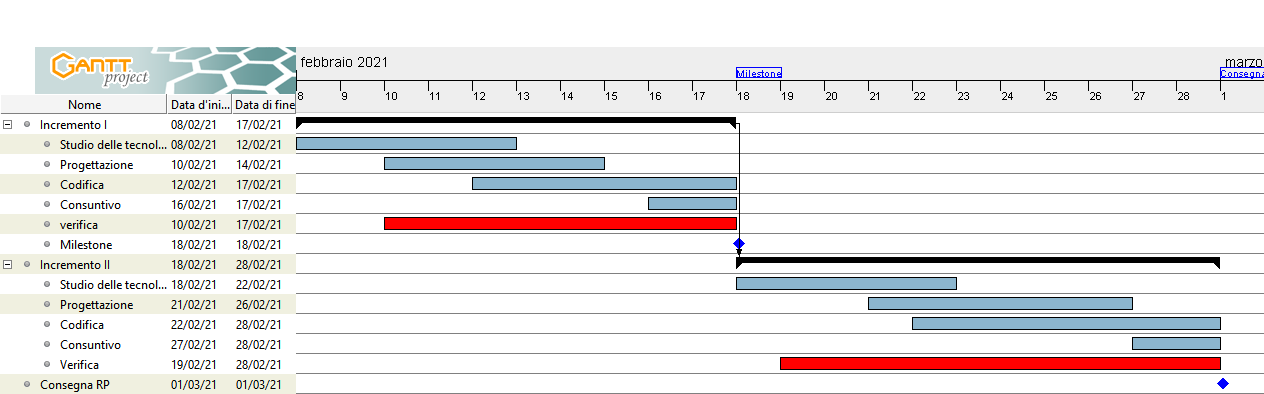
\includegraphics[width=\linewidth]{Images/GanttPianificazioneProgettazionePoc.PNG}
	\caption{Diagramma di Gantt dell'attività di progettazione e codifica del Proof Of Concept}
\end{figure}





\newpage
\subsection{Progettazione di dettaglio e codifica}
Questa fase comincia in seguito a quella precedente e termina con la \textit{Revisione di Qualifica}, ovvero dal 08-03-2021 al 02-04-2021. Durante questa fase verranno implementate buona parte delle componenti della web app e verranno anche aggiunte funzionalità alle componenti già sviluppate in precedenza.
Di seguito è riportato il dettaglio di ogni incremento.

\subsubsection{Incremento III}
\textit{dal 08-03-2021 al 13-03-2021}\\
L'incremento III prevede la progettazione di dettaglio e codifica delle componenti software. Si prevede di svolgere quanto segue:
\begin{itemize}
\item Implementazione di un componente per applicare una riduzione dimensionale ai dati;
\item Aggiunta di alcuni controlli per la configurazione dei parametri relativi ai diversi algoritmi di riduzione dimensionale disponibili.
\end{itemize}
\textbf{Attività}
\begin{itemize}
\item \textbf{Stesura:} eventuali correzioni ai documenti ed inizio stesura dell'allegato tecnico con scelta dei design patterns;
\item \textbf{Verifica documenti}
\item \textbf{Progettazione:} progettazione del componente per la riduzione dimensionale;
\item \textbf{Codifica:} codifica del componente per la riduzione dimensionale con relativa parametrizzazione;
\item \textbf{Verifica software:} verifica sulle funzionalità software aggiunte.
\end{itemize}
\subsubsection{Incremento IV}
\textit{dal 13-03-2021 al 17-03-2021}\\
L'incremento IV prevede la progettazione di dettaglio e codifica delle componenti software. Si prevede di svolgere quanto segue:
\begin{itemize}
\item Implementazione della visualizzazione Heat Map;
\item Aggiunta di alcuni controlli per la configurazione dei parametri relativi alla visualizzazione precedentemente implementata.
\end{itemize}
\textbf{Attività}
\begin{itemize}
\item \textbf{Stesura:} incremento della documentazione da allegare al prodotto;
\item \textbf{Verifica documenti}
\item \textbf{Progettazione:} progettazione del componente per la visualizzazione Heat Map;
\item \textbf{Codifica:} codifica del componente per la visualizzazione con relativa parametrizzazione;
\item \textbf{Verifica software:} verifica sulle funzionalità software aggiunte.
\end{itemize}

\subsubsection{Incremento V}
\textit{dal 17-03-2021 al 21-03-2021}\\
L'incremento V prevede la progettazione di dettaglio e codifica delle componenti software. Si prevede di svolgere quanto segue:
\begin{itemize}
\item Implementazione della visualizzazione Force Field;
\item Aggiunta di alcuni controlli per la configurazione dei parametri relativi alla visualizzazione precedentemente implementata.
\end{itemize}
\textbf{Attività}
\begin{itemize}
\item \textbf{Stesura:} incremento della documentazione da allegare al prodotto e inizio del manuale utente e del manuale manutentore;
\item \textbf{Verifica documenti}
\item \textbf{Progettazione:} progettazione del componente per la visualizzazione Force Field;
\item \textbf{Codifica:} codifica del componente per la visualizzazione con relativa parametrizzazione;
\item \textbf{Verifica software:} verifica sulle funzionalità software aggiunte.
\end{itemize}

\subsubsection{Incremento VI}
\textit{dal 21-03-2021 al 26-03-2021}\\
L'incremento V prevede la progettazione di dettaglio e codifica delle componenti software. Si prevede di svolgere quanto segue:
\begin{itemize}
\item Implementazione della visualizzazione Proiezione Lineare Multi Asse;
\item Aggiunta di alcuni controlli per la configurazione dei parametri relativi alla visualizzazione precedentemente implementata.
\end{itemize}
\textbf{Attività}
\begin{itemize}
\item \textbf{Stesura:} incremento della documentazione da allegare al prodotto ;
\item \textbf{Verifica documenti}
\item \textbf{Progettazione:} progettazione del componente per la visualizzazione Proiezione Lineare Multi Asse;
\item \textbf{Codifica:} codifica del componente per la visualizzazione con relativa parametrizzazione;
\item \textbf{Verifica software:} verifica sulle funzionalità software aggiunte.
\end{itemize}

\subsubsection{Incremento VII}
\textit{dal 26-03-2021 al 2-04-2021}\\
L'incremento V prevede la progettazione di dettaglio e codifica delle componenti software. Si prevede di svolgere quanto segue:
\begin{itemize}
\item Implementazione di un database;
\item Sviluppo di un componente per la scelta e il caricamento di un dataset contenuto nel database.
\end{itemize}
\textbf{Attività}
\begin{itemize}
\item \textbf{Stesura:} incremento e conclusione della documentazione da allegare al prodotto ;
\item \textbf{Verifica documenti}
\item \textbf{Progettazione:} progettazione del database e del componente per la scelta e il caricamento del dataset;
\item \textbf{Creazione struttura database:} stesura della struttura del database;
\item \textbf{Codifica:} codifica del componente per la scelta e il caricamento del dataset;
\item \textbf{Verifica software:} verifica sulle funzionalità software aggiunte.
\end{itemize}

\begin{landscape}

\begin{figure}[h]
 	\centering
	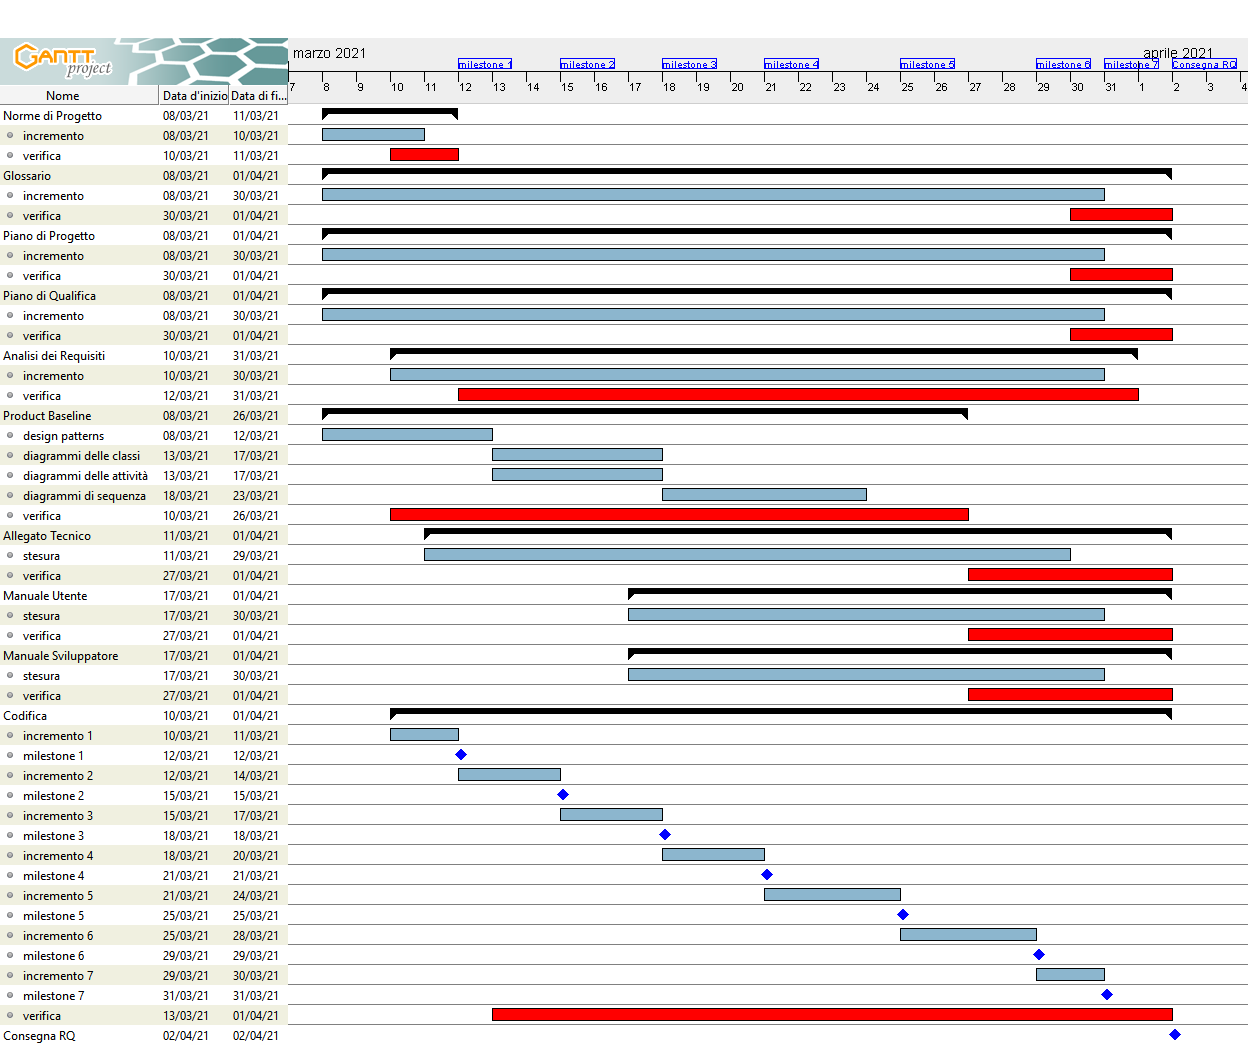
\includegraphics[width=\linewidth]{Images/GanttPianificazioneProgettazioneDettaglioCodifica.png}
	\caption{Diagramma di Gantt dell'attività di Progettazione di dettaglio e Codifica}
\end{figure}

\end{landscape}
\newpage
\subsection{Completamento e raffinamento delle funzionalità}
Questa fase comincia subito dopo la consegna dei documenti per la \textit{Revisione di Qualifica}, ovvero il 26-04-2021 e termina il 30-04-2021.\\
In questo periodo verranno creati ulteriori test per verificare il corretto funzionamento del prodotto. Se tutte le scadenze imposte dal gruppo vengono rispettate il tempo in eccesso viene occupato per la realizzazione di requisiti opzionali, concordati con il proponente. 

\subsubsection{Incremento VIII} 

\paragraph{Obiettivi}
\begin{itemize}
	\item Implementazione della gestione della sessione;
	\item Implementazione di un componente per l'esportazione dei parametri di configurazione dell'applicazione \textbf{[UC7]};
	\item Implementazione di un componente per l'importazione dei parametri di configurazione dell'applicazione \textbf{[UC1.2]}.
\end{itemize}
	
\paragraph{Periodi e attività} \mbox{}\\\mbox{}\\
Questo incremento si compone di un unico periodo, dal  26-04-2021 al 30-04-2021, con milestone fissata per l'ultimo giorno. Comprende attività di:	
\begin{itemize}
\item \textbf{Stesura:} incremento della documentazione da allegare al prodotto;
\item \textbf{Verifica dei documenti};
\item \textbf{Progettazione:} progettazione di un sistema per la gestione della sessione;
\item \textbf{Codifica:} codifica dei componenti per l'importazione e l'esportazione dei parametri di configurazione dell'applicazione;
\item \textbf{Verifica software:} verifica sulle funzionalità software aggiunte.
\end{itemize}
%
%\subsubsection{Incremento IX} 
%
%\paragraph{Obiettivi}
%\begin{itemize}
%	\item Implementazione di un sistema di \glo{widget} per l'utilizzo dell'applicazione;
%	\item Realizzazione una guida introduttiva per l'utilizzo dell'applicazione.
%\end{itemize}			
%\paragraph{Periodi e attività} \mbox{}\\\mbox{}\\
%Questo incremento si compone di un unico periodo, dal  16-04-2021 al 23-04-2021, con milestone fissata per l'ultimo giorno.		
%\begin{itemize}
%\item \textbf{Stesura:} incremento della documentazione da allegare al prodotto;
%\item \textbf{Verifica dei documenti} 
%\item \textbf{Progettazione:} progettazione di un sistema di \glo{widget} e di una guida introduttiva;
%\item \textbf{Codifica:} codifica dei componenti per i \glo{widget} e per la guida introduttiva;
%\item \textbf{Verifica software:} verifica sulle funzionalità software aggiunte.
%\end{itemize}

\begin{figure}[h]
	\centering
	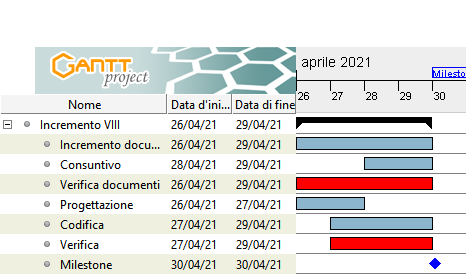
\includegraphics[width=12cm]{Images/GanttPianificazioneRaffinamentoFunzionalita.PNG}
	\caption{Diagramma di Gantt dell'attività di completamento e raffinamento delle funzionalità}
\end{figure}
\newpage
\subsection{Validazione e Collaudo}
Questa fase comincia subito dopo la fase precedente e finisce con la data di consegna per la \textit{Revisione di Accettazione}, ovvero dal 09-04-2020 al 03-05-2020.\\
In questo periodo verranno creati ulteriori test per verificare il corretto funzionamento del prodotto. Se tutte le scadenze imposte dal gruppo vengono rispettate il tempo in eccesso viene occupato per la realizzazione di requisiti opzionali, concordati con il committente. 
\subsubsection{Attività}
\begin{itemize}
\item \textbf{Incremento e verifica dei documenti:} se fosse necessario, i documenti prodotti dal team verranno integrati.

 \item \textbf{Incremento e verifica delle attività}: sia la \textit{Technology baseline} che la \textit{Product Baseline} vengono eventualmente raffinate; particolare attenzione va alla codifica, svolta ad incrementi ciclici.
 \begin{itemize}
 \item \textbf{Incremento X}: il gruppo identifica e implementa la soluzione più adeguata per la gestione della sessione nell'applicazione. Incremento della documentazione da correlare al prodotto software e incremento della documentazione per verifica e miglioramento continuo \textbf{[UC1.2, UC7]};
\item \textbf{Incremento XI}: viene perfezionato il codice precedentemente, il prodotto viene collaudato e vengono vericati tutti i documenti precedentemente redatti. 
 \end{itemize}

 \item \textbf{Verifica e collaudo}: vengono creati e applicati un set di test, che hanno lo scopo di portare il prodotto ad un buon livello qualitativo. Il gruppo si focalizzerà sulla sua correttezza e nel rispetto di tutti i requisiti.
\end{itemize}

\subsubsection{Periodi}
La pianificazione di questa fase è stata organizzata con le seguenti milestone:

\begin{itemize}
\item \textbf{Periodo 1}: \textit{(dal 09-04-2020 al 16-04-2020)} se fosse necessario, in questo periodo viene controllata tutta la documentazione e ci si dedicherà ad eventuali incrementi della \textit{Technology Baseline} e \textit{Product Baseline}, è fissata una milestone l'ultimo giorno di questo periodo entra cui dovrà essere terminato l'incremento X.

\item \textbf{Periodo 2}: \textit{(dal 16-04-2020 al 03-05-2020)} entro la milestone del 03-05-2020 il gruppo ha come obbiettivo quello di completare l'ultimo incremento.

\end{itemize}
\newpage
\subsubsection{Diagramma di Gantt: Validazione e Collaudo}
\begin{figure}[h]
	\centering
	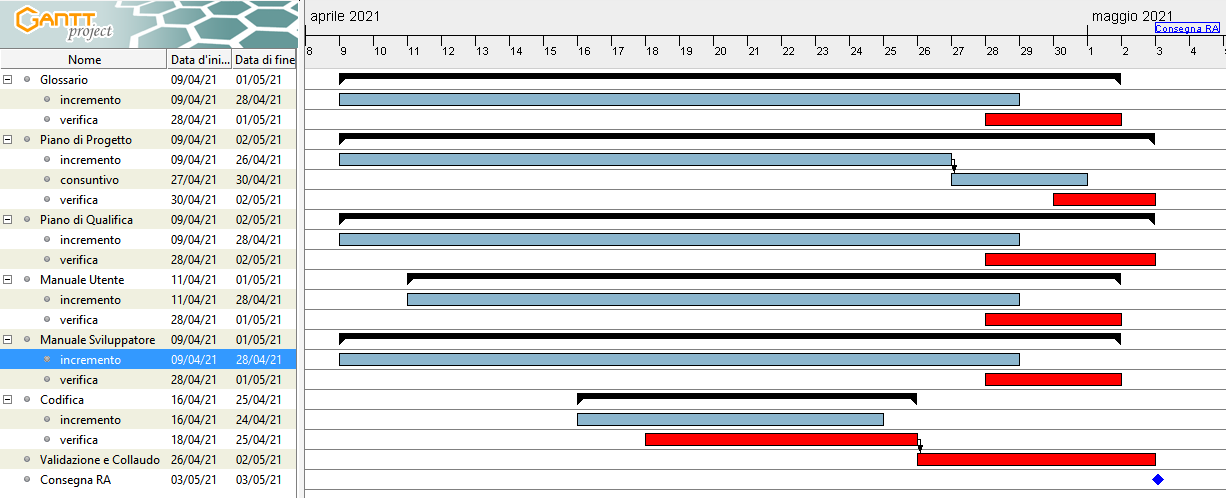
\includegraphics[scale=0.5]{Images/GanttValidazioneCollaudo.PNG}
	\caption{Diagramma di Gantt dell'attività di Validazione e Collaudo}
\end{figure}
\newpage
\section{Preventivo}
In questa sezione viene esposta la ripartizione delle risorse disponibili tra i membri del gruppo \Gruppo{}. Per le sigle utilizzate per l'identificazione dei ruoli si vedano le \NdPv{}.
\subsection{Fase di Analisi}
Di seguito vengono riportate le tabelle della distribuzione oraria in questa fase e i costi da affrontare per ogni ruolo.
\subsubsection{Prospetto orario ed economico}

\begin{minipage}[b]{0.2\linewidth}

\begin{longtable}{ c | c c c c c c | c} 
 	\rowcolor{coloreRosso}
 	\color{white}{\textbf{Nominativo}} &
 	\color{white}{\textbf{RE}} &
 	\color{white}{\textbf{AM}} &
 	\color{white}{\textbf{AN}} &
 	\color{white}{\textbf{PT}} &
 	\color{white}{\textbf{PR}} &
 	\color{white}{\textbf{VE}} &
 	\color{white}{\textbf{Tot.}} \\
   
 \BM{} & 14 & - & 12 & - & - & 4 & 30 \\ 
 \SG{} & 11 & - & 13 & - & - & 6 & 30 \\ 
 \SH{} & - & 7 & 17 & - & - & 6 & 30 \\ 
 \PA{} & - & 14 & 2 & - & - & 14 & 30 \\ 
 \SP{} & - & - & 22 & - & - & 8 & 30 \\ 
 \RA{} & - & 12 & 4 & - & - & 14 & 30 \\ 
 \ZM{} & - & 12 & 8 & - & - & 10 & 30 \\ 
 
 	\rowcolor{coloreRosso}
 	\color{white}{\textbf{Totale ore ruolo}} &
 	\color{white}{\textbf{25}} &
 	\color{white}{\textbf{45}} &
 	\color{white}{\textbf{78}} &
 	\color{white}{\textbf{0}} &
 	\color{white}{\textbf{0}} &
 	\color{white}{\textbf{62}} &
 	\color{white}{\textbf{210}} \\ 	
 	\rowcolor{white}
 	\caption{\parbox{7cm}{Distribuizione delle ore nel periodo di Analisi}}
\end{longtable}

\end{minipage}
\begin{minipage}[b]{1.25\linewidth}

\begin{longtable}{ c | c | c} 
 	\rowcolor{coloreRosso}
 	\color{white}{\textbf{Ruolo}} &
 	\color{white}{\textbf{Ore}} &
 	\color{white}{\textbf{Costo €}} \\
 	
 	Responsabile & 25 & 750\\
 	Amministratore & 45 & 900\\
 	Analista & 78 & 1950\\
 	Progettista & - & -\\
 	Programmatore & - & -\\
 	Verificatore & 62 & 930\\
 	
 	\rowcolor{coloreRosso}
 	\color{white}{\textbf{Totale}} &
 	\color{white}{\textbf{210}} &
 	\color{white}{\textbf{4530}}\\
 	\rowcolor{white}
 	\caption{\parbox{5cm}{Prospetto dei costi per ruolo nel periodo di Analisi }}
\end{longtable}
\end{minipage}

\subsection{Fase di progettazione architetturale}
\subsubsection{Prospetto orario ed economico}

\begin{minipage}[b]{0.2\linewidth}

\begin{longtable}{ c | c c c c c c | c} 
 \rowcolor{coloreRosso}
 \color{white}{\textbf{Nominativo}} &
 \color{white}{\textbf{RE}} &
 \color{white}{\textbf{AM}} &
 \color{white}{\textbf{AN}} &
 \color{white}{\textbf{PT}} &
 \color{white}{\textbf{PR}} &
 \color{white}{\textbf{VE}} &
 \color{white}{\textbf{Tot.}} \\
 	
 \BM{} & - & 9 & 7 & 9 & 3 & 4 & 32 \\ 
 \SG{} & - & 9 & 5 & 9 & 4 & 5 & 32 \\ 
 \SH{} & - & - & 5 & 9 & 8 & 10 & 32 \\ 
 \PA{} & 6 & - & 5 & 7 & 5 & 9 & 32 \\ 
 \SP{} & - & 12 & - & 8 & 6 & 6 & 32 \\ 
 \RA{} & - & - & 11 & 8 & 6 & 7 & 32 \\ 
 \ZM{} & 6 & - & 10 & 10 & 2 & 4 & 32 \\
 
 	\rowcolor{coloreRosso}
 	\color{white}{\textbf{Totale ore ruolo}} &
 	\color{white}{\textbf{12}} &
 	\color{white}{\textbf{30}} &
 	\color{white}{\textbf{43}} &
 	\color{white}{\textbf{60}} &
 	\color{white}{\textbf{34}} &
 	\color{white}{\textbf{45}} &
 	\color{white}{\textbf{224}} \\
	\rowcolor{white}
 	\caption{Distribuizione delle ore nel periodo di Progettazione architetturale}
\end{longtable}

\end{minipage}
\begin{minipage}[b]{1.25\linewidth}

\begin{longtable}{ c | c | c} 
 	\rowcolor{coloreRosso}
 	\color{white}{\textbf{Ruolo}} &
 	\color{white}{\textbf{Ore}} &
 	\color{white}{\textbf{Costo €}} \\
 	
 	Responsabile & 12 & 360\\
 	Amministratore & 30 & 600\\
 	Analista & 43 & 1075\\
 	Progettista & 60 & 1320\\
 	Programmatore & 34 & 510\\
 	Verificatore & 45 & 675\\
 	
 	\rowcolor{coloreRosso}
 	\color{white}{\textbf{Totale}} &
 	\color{white}{\textbf{224}} &
 	\color{white}{\textbf{4540}}\\
 	\rowcolor{white}
 	\caption{\parbox{5cm}{Prospetto dei costi per ruolo nel periodo di Progettazione architetturale}}	
\end{longtable}
\end{minipage}
\subsection{Fase di progettazione di dettaglio e codifica}
Di seguito vengono riportate le tabelle della distribuzione oraria in questa fase e i costi da affrontare per ogni ruolo.
\subsubsection{Incremento I}

I dati riportati di seguito si riferiscono al periodo che va dal 08-03-2020 al 10-03-2020.

\begin{minipage}[b]{0.65\linewidth}
\begin{small}

\begin{longtable}{ c | c c c c c c | c} 
 \rowcolor{coloreRosso}
 \color{white}{\textbf{Nominativo}} &
 \color{white}{\textbf{RE}} &
 \color{white}{\textbf{AM}} &
 \color{white}{\textbf{AN}} &
 \color{white}{\textbf{PT}} &
 \color{white}{\textbf{PR}} &
 \color{white}{\textbf{VE}} &
 \color{white}{\textbf{Tot.}} \\
 	
 \BM{} & - & 2 & 2 & 4 & - & 4 & 12 \\ 
 \PA{} & 4 & - & 5 & 3 & - & - & 12 \\ 
 \RA{} & - & - & 5 & - & 4 & 5 & 10 \\ 
 \SH{} & - & - & 2 & 5 & - & 3 & 14 \\ 
 \SG{} & - & 3 & - & 4 & - & 5 & 12 \\ 
 \SP{} & - & 3 & - & 5 & - & 6 & 14 \\ 
 \ZM{} & - & - & 5 & 3 & - & 4 & 12 \\
 
 	\rowcolor{coloreRosso}
 	\color{white}{\textbf{Totale ore ruolo}} &
 	\color{white}{\textbf{4}} &
 	\color{white}{\textbf{8}} &
 	\color{white}{\textbf{19}} &
 	\color{white}{\textbf{24}} &
 	\color{white}{\textbf{4}} &
 	\color{white}{\textbf{27}} &
 	\color{white}{\textbf{86}} \\
	\rowcolor{white}
	\captionsetup{width=.9\textwidth}
 	\caption{Distribuzione delle ore nel periodo I della Progettazione architetturale}
\end{longtable}

\end{small}
\end{minipage}
\begin{minipage}[b]{.3\linewidth}
\begin{small}

\begin{longtable}{ c | c | c} 
 	\rowcolor{coloreRosso}
 	\color{white}{\textbf{Ruolo}} &
 	\color{white}{\textbf{Ore}} &
 	\color{white}{\textbf{Costo €}} \\
 	
 	Responsabile & 4 & 120\\
 	Amministratore & 8 & 160\\
 	Analista & 19 & 475\\
 	Progettista & 24 & 528\\
 	Programmatore & 4 & 60\\
 	Verificatore & 27 & 405\\
 	
 	\rowcolor{coloreRosso}
 	\color{white}{\textbf{Totale}} &
 	\color{white}{\textbf{86}} &
 	\color{white}{\textbf{1748}}\\
 	\rowcolor{white}
 	\caption{Costi per ruolo nel periodo I della Progettazione architetturale}
\end{longtable}

\end{small}
\end{minipage}

\subsubsection{Incremento II}

I dati riportati di seguito si riferiscono al periodo che va dall' 10-03-2020 al 12-02-2020.

\begin{minipage}[b]{0.65\linewidth}
\begin{small}

\begin{longtable}{ c | c c c c c c | c} 
 \rowcolor{coloreRosso}
 \color{white}{\textbf{Nominativo}} &
 \color{white}{\textbf{RE}} &
 \color{white}{\textbf{AM}} &
 \color{white}{\textbf{AN}} &
 \color{white}{\textbf{PT}} &
 \color{white}{\textbf{PR}} &
 \color{white}{\textbf{VE}} &
 \color{white}{\textbf{Tot.}} \\
 	
 \BM{} & - & 4 & 3 & 5 & - & - & 12 \\ 
 \PA{} & 2 & - & - & - & 5 & 4 & 11 \\ 
 \RA{} & - & - & 6 & 2 & 2 & 2 & 12 \\ 
 \SH{} & - & - & 3 & 2 & 1 & 3 & 9 \\ 
 \SG{} & - & 5 & 3 & 5 & - & - & 13 \\ 
 \SP{} & - & 3 & - & 3 & 6 & - & 12 \\ 
 \ZM{} & - & - & 5 & 7 & - & - & 12 \\
 
 	\rowcolor{coloreRosso}
 	\color{white}{\textbf{Totale ore ruolo}} &
 	\color{white}{\textbf{2}} &
 	\color{white}{\textbf{12}} &
 	\color{white}{\textbf{20}} &
 	\color{white}{\textbf{24}} &
 	\color{white}{\textbf{14}} &
 	\color{white}{\textbf{9}} &
 	\color{white}{\textbf{81}} \\
	\rowcolor{white}
	\captionsetup{width=.9\textwidth}
 	\caption{Distribuzione delle ore nel periodo II della Progettazione architetturale}
\end{longtable}

\end{small}
\end{minipage}
\begin{minipage}[b]{.3\linewidth}
\begin{small}

\begin{longtable}{ c | c | c} 
 	\rowcolor{coloreRosso}
 	\color{white}{\textbf{Ruolo}} &
 	\color{white}{\textbf{Ore}} &
 	\color{white}{\textbf{Costo €}} \\
 	
 	Responsabile & 2 & 60\\
 	Amministratore & 12 & 240\\
 	Analista & 20 & 500\\
 	Progettista & 24 & 528\\
 	Programmatore & 14 & 210\\
 	Verificatore & 9 & 135\\
 	
 	\rowcolor{coloreRosso}
 	\color{white}{\textbf{Totale}} &
 	\color{white}{\textbf{81}} &
 	\color{white}{\textbf{1673}}\\
 	\rowcolor{white}
 	\caption{Costi per ruolo nel periodo II della Progettazione architetturale}
\end{longtable}

\end{small}
\end{minipage}

\subsubsection{Incremento III}

I dati riportati di seguito si riferiscono al periodo che va dal 18-02-2020 al 01-03-2020.

\begin{minipage}[b]{0.65\linewidth}
\begin{small}

\begin{longtable}{ c | c c c c c c | c} 
 \rowcolor{coloreRosso}
 \color{white}{\textbf{Nominativo}} &
 \color{white}{\textbf{RE}} &
 \color{white}{\textbf{AM}} &
 \color{white}{\textbf{AN}} &
 \color{white}{\textbf{PT}} &
 \color{white}{\textbf{PR}} &
 \color{white}{\textbf{VE}} &
 \color{white}{\textbf{Tot.}} \\
 	
 \BM{} & - & 3 & 2 & - & 3 & - & 8 \\ 
 \PA{} & - & - & - & 4 & - & 5 & 9 \\ 
 \RA{} & - & - & - & 6 & 4 & - & 10 \\ 
 \SH{} & - & - & - & 2 & 3 & 4 & 9 \\ 
 \SG{} & - & 1 & 2 & - & 4 & - & 7 \\ 
 \SP{} & - & 6 & - & - & - & - & 6 \\ 
 \ZM{} & 6 & - & - & - & 2 & - & 8 \\
 
 	\rowcolor{coloreRosso}
 	\color{white}{\textbf{Totale ore ruolo}} &
 	\color{white}{\textbf{6}} &
 	\color{white}{\textbf{10}} &
 	\color{white}{\textbf{4}} &
 	\color{white}{\textbf{12}} &
 	\color{white}{\textbf{16}} &
 	\color{white}{\textbf{9}} &
 	\color{white}{\textbf{57}} \\
	\rowcolor{white}
	\captionsetup{width=.9\textwidth}
 	\caption{Distribuzione delle ore nel periodo III della Progettazione architetturale}
\end{longtable}

\end{small}
\end{minipage}
\begin{minipage}[b]{.3\linewidth}
\begin{small}

\begin{longtable}{ c | c | c} 
 	\rowcolor{coloreRosso}
 	\color{white}{\textbf{Ruolo}} &
 	\color{white}{\textbf{Ore}} &
 	\color{white}{\textbf{Costo €}} \\
 	
 	Responsabile & 6 & 180\\
 	Amministratore & 10 & 200\\
 	Analista & 4 & 100\\
 	Progettista & 12 & 264\\
 	Programmatore & 16 & 240\\
 	Verificatore & 9 & 135\\
 	
 	\rowcolor{coloreRosso}
 	\color{white}{\textbf{Totale}} &
 	\color{white}{\textbf{57}} &
 	\color{white}{\textbf{1119}}\\
 	\rowcolor{white}
 	\caption{Costi per ruolo nel periodo III della Progettazione architetturale}
\end{longtable}

\end{small}
\end{minipage}

\subsubsection{Incremento IV}

I dati riportati di seguito si riferiscono al periodo che va dal 18-02-2020 al 01-03-2020.

\begin{minipage}[b]{0.65\linewidth}
\begin{small}

\begin{longtable}{ c | c c c c c c | c} 
 \rowcolor{coloreRosso}
 \color{white}{\textbf{Nominativo}} &
 \color{white}{\textbf{RE}} &
 \color{white}{\textbf{AM}} &
 \color{white}{\textbf{AN}} &
 \color{white}{\textbf{PT}} &
 \color{white}{\textbf{PR}} &
 \color{white}{\textbf{VE}} &
 \color{white}{\textbf{Tot.}} \\
 	
 \BM{} & - & 3 & 2 & - & 3 & - & 8 \\ 
 \PA{} & - & - & - & 4 & - & 5 & 9 \\ 
 \RA{} & - & - & - & 6 & 4 & - & 10 \\ 
 \SH{} & - & - & - & 2 & 3 & 4 & 9 \\ 
 \SG{} & - & 1 & 2 & - & 4 & - & 7 \\ 
 \SP{} & - & 6 & - & - & - & - & 6 \\ 
 \ZM{} & 6 & - & - & - & 2 & - & 8 \\
 
 	\rowcolor{coloreRosso}
 	\color{white}{\textbf{Totale ore ruolo}} &
 	\color{white}{\textbf{6}} &
 	\color{white}{\textbf{10}} &
 	\color{white}{\textbf{4}} &
 	\color{white}{\textbf{12}} &
 	\color{white}{\textbf{16}} &
 	\color{white}{\textbf{9}} &
 	\color{white}{\textbf{57}} \\
	\rowcolor{white}
	\captionsetup{width=.9\textwidth}
 	\caption{Distribuzione delle ore nel periodo III della Progettazione architetturale}
\end{longtable}

\end{small}
\end{minipage}
\begin{minipage}[b]{.3\linewidth}
\begin{small}

\begin{longtable}{ c | c | c} 
 	\rowcolor{coloreRosso}
 	\color{white}{\textbf{Ruolo}} &
 	\color{white}{\textbf{Ore}} &
 	\color{white}{\textbf{Costo €}} \\
 	
 	Responsabile & 6 & 180\\
 	Amministratore & 10 & 200\\
 	Analista & 4 & 100\\
 	Progettista & 12 & 264\\
 	Programmatore & 16 & 240\\
 	Verificatore & 9 & 135\\
 	
 	\rowcolor{coloreRosso}
 	\color{white}{\textbf{Totale}} &
 	\color{white}{\textbf{57}} &
 	\color{white}{\textbf{1119}}\\
 	\rowcolor{white}
 	\caption{Costi per ruolo nel periodo III della Progettazione architetturale}
\end{longtable}

\end{small}
\end{minipage}

\subsubsection{Incremento V}

I dati riportati di seguito si riferiscono al periodo che va dal 18-02-2020 al 01-03-2020.

\begin{minipage}[b]{0.65\linewidth}
\begin{small}

\begin{longtable}{ c | c c c c c c | c} 
 \rowcolor{coloreRosso}
 \color{white}{\textbf{Nominativo}} &
 \color{white}{\textbf{RE}} &
 \color{white}{\textbf{AM}} &
 \color{white}{\textbf{AN}} &
 \color{white}{\textbf{PT}} &
 \color{white}{\textbf{PR}} &
 \color{white}{\textbf{VE}} &
 \color{white}{\textbf{Tot.}} \\
 	
 \BM{} & - & 3 & 2 & - & 3 & - & 8 \\ 
 \PA{} & - & - & - & 4 & - & 5 & 9 \\ 
 \RA{} & - & - & - & 6 & 4 & - & 10 \\ 
 \SH{} & - & - & - & 2 & 3 & 4 & 9 \\ 
 \SG{} & - & 1 & 2 & - & 4 & - & 7 \\ 
 \SP{} & - & 6 & - & - & - & - & 6 \\ 
 \ZM{} & 6 & - & - & - & 2 & - & 8 \\
 
 	\rowcolor{coloreRosso}
 	\color{white}{\textbf{Totale ore ruolo}} &
 	\color{white}{\textbf{6}} &
 	\color{white}{\textbf{10}} &
 	\color{white}{\textbf{4}} &
 	\color{white}{\textbf{12}} &
 	\color{white}{\textbf{16}} &
 	\color{white}{\textbf{9}} &
 	\color{white}{\textbf{57}} \\
	\rowcolor{white}
	\captionsetup{width=.9\textwidth}
 	\caption{Distribuzione delle ore nel periodo III della Progettazione architetturale}
\end{longtable}

\end{small}
\end{minipage}
\begin{minipage}[b]{.3\linewidth}
\begin{small}

\begin{longtable}{ c | c | c} 
 	\rowcolor{coloreRosso}
 	\color{white}{\textbf{Ruolo}} &
 	\color{white}{\textbf{Ore}} &
 	\color{white}{\textbf{Costo €}} \\
 	
 	Responsabile & 6 & 180\\
 	Amministratore & 10 & 200\\
 	Analista & 4 & 100\\
 	Progettista & 12 & 264\\
 	Programmatore & 16 & 240\\
 	Verificatore & 9 & 135\\
 	
 	\rowcolor{coloreRosso}
 	\color{white}{\textbf{Totale}} &
 	\color{white}{\textbf{57}} &
 	\color{white}{\textbf{1119}}\\
 	\rowcolor{white}
 	\caption{Costi per ruolo nel periodo III della Progettazione architetturale}
\end{longtable}

\end{small}
\end{minipage}
\subsubsection{Incremento VI}

I dati riportati di seguito si riferiscono al periodo che va dal 18-02-2020 al 01-03-2020.

\begin{minipage}[b]{0.65\linewidth}
\begin{small}

\begin{longtable}{ c | c c c c c c | c} 
 \rowcolor{coloreRosso}
 \color{white}{\textbf{Nominativo}} &
 \color{white}{\textbf{RE}} &
 \color{white}{\textbf{AM}} &
 \color{white}{\textbf{AN}} &
 \color{white}{\textbf{PT}} &
 \color{white}{\textbf{PR}} &
 \color{white}{\textbf{VE}} &
 \color{white}{\textbf{Tot.}} \\
 	
 \BM{} & - & 3 & 2 & - & 3 & - & 8 \\ 
 \PA{} & - & - & - & 4 & - & 5 & 9 \\ 
 \RA{} & - & - & - & 6 & 4 & - & 10 \\ 
 \SH{} & - & - & - & 2 & 3 & 4 & 9 \\ 
 \SG{} & - & 1 & 2 & - & 4 & - & 7 \\ 
 \SP{} & - & 6 & - & - & - & - & 6 \\ 
 \ZM{} & 6 & - & - & - & 2 & - & 8 \\
 
 	\rowcolor{coloreRosso}
 	\color{white}{\textbf{Totale ore ruolo}} &
 	\color{white}{\textbf{6}} &
 	\color{white}{\textbf{10}} &
 	\color{white}{\textbf{4}} &
 	\color{white}{\textbf{12}} &
 	\color{white}{\textbf{16}} &
 	\color{white}{\textbf{9}} &
 	\color{white}{\textbf{57}} \\
	\rowcolor{white}
	\captionsetup{width=.9\textwidth}
 	\caption{Distribuzione delle ore nel periodo III della Progettazione architetturale}
\end{longtable}

\end{small}
\end{minipage}
\begin{minipage}[b]{.3\linewidth}
\begin{small}

\begin{longtable}{ c | c | c} 
 	\rowcolor{coloreRosso}
 	\color{white}{\textbf{Ruolo}} &
 	\color{white}{\textbf{Ore}} &
 	\color{white}{\textbf{Costo €}} \\
 	
 	Responsabile & 6 & 180\\
 	Amministratore & 10 & 200\\
 	Analista & 4 & 100\\
 	Progettista & 12 & 264\\
 	Programmatore & 16 & 240\\
 	Verificatore & 9 & 135\\
 	
 	\rowcolor{coloreRosso}
 	\color{white}{\textbf{Totale}} &
 	\color{white}{\textbf{57}} &
 	\color{white}{\textbf{1119}}\\
 	\rowcolor{white}
 	\caption{Costi per ruolo nel periodo III della Progettazione architetturale}
\end{longtable}

\end{small}
\end{minipage}
\subsubsection{Incremento VII}

I dati riportati di seguito si riferiscono al periodo che va dal 18-02-2020 al 01-03-2020.

\begin{minipage}[b]{0.65\linewidth}
\begin{small}

\begin{longtable}{ c | c c c c c c | c} 
 \rowcolor{coloreRosso}
 \color{white}{\textbf{Nominativo}} &
 \color{white}{\textbf{RE}} &
 \color{white}{\textbf{AM}} &
 \color{white}{\textbf{AN}} &
 \color{white}{\textbf{PT}} &
 \color{white}{\textbf{PR}} &
 \color{white}{\textbf{VE}} &
 \color{white}{\textbf{Tot.}} \\
 	
 \BM{} & - & 3 & 2 & - & 3 & - & 8 \\ 
 \PA{} & - & - & - & 4 & - & 5 & 9 \\ 
 \RA{} & - & - & - & 6 & 4 & - & 10 \\ 
 \SH{} & - & - & - & 2 & 3 & 4 & 9 \\ 
 \SG{} & - & 1 & 2 & - & 4 & - & 7 \\ 
 \SP{} & - & 6 & - & - & - & - & 6 \\ 
 \ZM{} & 6 & - & - & - & 2 & - & 8 \\
 
 	\rowcolor{coloreRosso}
 	\color{white}{\textbf{Totale ore ruolo}} &
 	\color{white}{\textbf{6}} &
 	\color{white}{\textbf{10}} &
 	\color{white}{\textbf{4}} &
 	\color{white}{\textbf{12}} &
 	\color{white}{\textbf{16}} &
 	\color{white}{\textbf{9}} &
 	\color{white}{\textbf{57}} \\
	\rowcolor{white}
	\captionsetup{width=.9\textwidth}
 	\caption{Distribuzione delle ore nel periodo III della Progettazione architetturale}
\end{longtable}

\end{small}
\end{minipage}
\begin{minipage}[b]{.3\linewidth}
\begin{small}

\begin{longtable}{ c | c | c} 
 	\rowcolor{coloreRosso}
 	\color{white}{\textbf{Ruolo}} &
 	\color{white}{\textbf{Ore}} &
 	\color{white}{\textbf{Costo €}} \\
 	
 	Responsabile & 6 & 180\\
 	Amministratore & 10 & 200\\
 	Analista & 4 & 100\\
 	Progettista & 12 & 264\\
 	Programmatore & 16 & 240\\
 	Verificatore & 9 & 135\\
 	
 	\rowcolor{coloreRosso}
 	\color{white}{\textbf{Totale}} &
 	\color{white}{\textbf{57}} &
 	\color{white}{\textbf{1119}}\\
 	\rowcolor{white}
 	\caption{Costi per ruolo nel periodo III della Progettazione architetturale}
\end{longtable}

\end{small}
\end{minipage}

\subsubsection{Riepilogo}

\begin{minipage}[b]{0.65\linewidth}
\begin{small}

\begin{longtable}{ c | c c c c c c | c} 
 \rowcolor{coloreRosso}
 \color{white}{\textbf{Nominativo}} &
 \color{white}{\textbf{RE}} &
 \color{white}{\textbf{AM}} &
 \color{white}{\textbf{AN}} &
 \color{white}{\textbf{PT}} &
 \color{white}{\textbf{PR}} &
 \color{white}{\textbf{VE}} &
 \color{white}{\textbf{Tot.}} \\
 	
 \BM{} & - & 5 & - & 11 & 21 & 13 & 50 \\ 
 \SG{} & - & 6 & - & 13 & 21 & 10 & 50 \\ 
 \SH{} & 6 & 3 & - & 8 & 21 & 12 & 50 \\ 
 \PA{} & - & 4 & - & 10 & 21 & 15 & 50 \\ 
 \SP{} & 4 & 5 & - & 9 & 21 & 11 & 50 \\ 
 \RA{} & 4 & - & - & 15 & 21 & 10 & 50 \\ 
 \ZM{} & 6 & 4 & - & 9 & 21 & 10 & 50 \\
 
 \rowcolor{coloreRosso}
 	\color{white}{\textbf{Totale ore ruolo}} &
 	\color{white}{\textbf{20}} &
 	\color{white}{\textbf{27}} &
 	\color{white}{\textbf{-}} &
 	\color{white}{\textbf{75}} &
 	\color{white}{\textbf{147}} &
 	\color{white}{\textbf{81}} &
 	\color{white}{\textbf{350}} \\
 \rowcolor{white}
 \captionsetup{width=.9\textwidth}
 \caption{Distribuizione delle ore nel periodo di Progettazione di dettaglio e Codifica}
\end{longtable}

\end{small}
\end{minipage}
\begin{minipage}[b]{.3\linewidth}
\begin{small}

\begin{longtable}{ c | c | c} 
 	\rowcolor{coloreRosso}
 	\color{white}{\textbf{Ruolo}} &
 	\color{white}{\textbf{Ore}} &
 	\color{white}{\textbf{Costo €}} \\
 	
 	Responsabile & 20 & 600\\
 	Amministratore & 27 & 540\\
 	Analista & - & -\\
 	Progettista & 75 & 1650\\
 	Programmatore & 147 & 2205\\
 	Verificatore & 81 & 1215\\
 	
 	\rowcolor{coloreRosso}
 	\color{white}{\textbf{Totale}} &
 	\color{white}{\textbf{350}} &
 	\color{white}{\textbf{6210}}\\
 	\rowcolor{white}
 	\caption{Costi per ruolo nel periodo di Prog. di dettaglio e Codifica}
\end{longtable}

\end{small}
\end{minipage}

I seguenti grafici riassumo i dati ottenuti.

\begin{figure}[!htb]
   \begin{minipage}{0.6\textwidth}
     \centering
     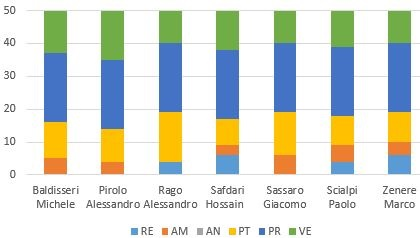
\includegraphics{Images/PO-Codifica}
     \caption{Ripartizione oraria per ciascun membro nella fase di Prog. di dettaglio e Codifica}
   \end{minipage}\hspace{0.1\textwidth}
   \begin{minipage}{0.3\textwidth}
     \centering
     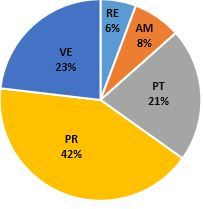
\includegraphics[width=.9\textwidth]{Images/PE-Codifica}
     \captionsetup{width=.9\textwidth}
     \caption{Ripartizione ore totali nella fase di Prog. di dettaglio e Codifica}
   \end{minipage}
\end{figure}

\subsection{Incremento VIII}
I dati riportati di seguito si riferiscono al periodo che va dal 26-04-2021 al 30-04-2021.

\begin{minipage}[b]{0.65\linewidth}
\begin{small}
{
\setlength\arrayrulewidth{1pt}
\begin{longtable}{ c | c c c c c c | c} 
 \rowcolor{coloreRosso}
 \color{white}{\textbf{Nominativo}} &
 \color{white}{\textbf{RE}} &
 \color{white}{\textbf{AM}} &
 \color{white}{\textbf{AN}} &
 \color{white}{\textbf{PT}} &
 \color{white}{\textbf{PR}} &
 \color{white}{\textbf{VE}} &
 \color{white}{\textbf{Tot.}} \\
 	
 \BM{} & - & 3 & - & - & 4 & 5 & 12 \\ 
 \PA{} & 4 & 2 & - & 1 & 2 & - & 9 \\ 
 \RA{} & 5 & - & - & - & - & 5 & 10 \\ 
 \SH{} & - & 3 & - & 1 & 3 & 3 & 10 \\ 
 \SG{} & - & - & - & - & 5 & 6 & 11 \\ 
 \SP{} & 2 & - & - & 1 & - & 8 & 11 \\ 
 \ZM{} & - & 2 & - & - & 2 & 6 & 10 \\
 
 	\rowcolor{coloreRosso}
 	\color{white}{\textbf{Totale ore ruolo}} &
 	\color{white}{\textbf{11}} &
 	\color{white}{\textbf{10}} &
 	\color{white}{\textbf{-}} &
 	\color{white}{\textbf{3}} &
 	\color{white}{\textbf{16}} &
 	\color{white}{\textbf{33}} &
 	\color{white}{\textbf{73}} \\
	\rowcolor{white}
	\captionsetup{width=.9\textwidth}
 	\caption{Distribuzione delle ore nell'incremento VIII}
\end{longtable}
}
\end{small}
\end{minipage}
\begin{minipage}[b]{.3\linewidth}
\begin{small}
{
\setlength\arrayrulewidth{1pt}
\begin{longtable}{ c | c | c} 
 	\rowcolor{coloreRosso}
 	\color{white}{\textbf{Ruolo}} &
 	\color{white}{\textbf{Ore}} &
 	\color{white}{\textbf{Costo €}} \\
 	
 	Responsabile & 11 & 330\\
 	Amministratore & 10 & 200\\
 	Analista & - & -\\
 	Progettista & 3 & 66\\
 	Programmatore & 16 & 240\\
 	Verificatore & 33 & 495\\
 	
 	\rowcolor{coloreRosso}
 	\color{white}{\textbf{Totale}} &
 	\color{white}{\textbf{73}} &
 	\color{white}{\textbf{1331 €}}\\
 	\rowcolor{white}
 	\caption{Costi per ruolo nell'incremento VIII}
\end{longtable}
}
\end{small}
\end{minipage}

\begin{figure}[!htb]   
    \centering
    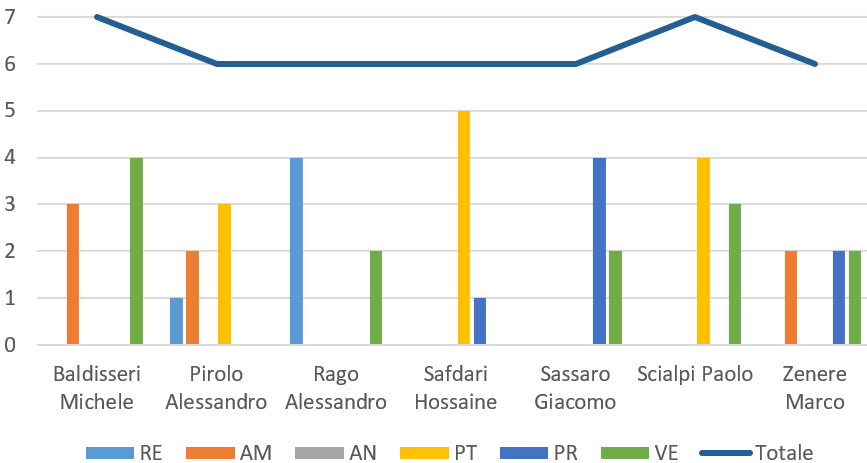
\includegraphics[width=0.90\textwidth]{Images/prev8}
	\caption{Ripartizione oraria per ciascun membro nell'incremento VIII}
\end{figure}


\subsection{Validazione e collaudo}

I dati riportati di seguito si riferiscono al periodo che va dal 01-05-2021 al 17-05-2021.

\begin{minipage}[b]{0.65\linewidth}
\begin{small}
{
\setlength\arrayrulewidth{1pt}
\begin{longtable}{ c | c c c c c c | c} 
 \rowcolor{coloreRosso}
 \color{white}{\textbf{Nominativo}} &
 \color{white}{\textbf{RE}} &
 \color{white}{\textbf{AM}} &
 \color{white}{\textbf{AN}} &
 \color{white}{\textbf{PT}} &
 \color{white}{\textbf{PR}} &
 \color{white}{\textbf{VE}} &
 \color{white}{\textbf{Tot.}} \\
 	
 \BM{} & - & - & - & - & - & 6 & 6 \\ 
 \PA{} & 2 & 2 & - & - & 2 & - & 6 \\ 
 \RA{} & 3 & 4 & - & - & - & 1 & 8 \\ 
 \SH{} & - & - & - & - & 4 & 2 & 6 \\ 
 \SG{} & - & - & - & - & 2 & 5 & 7 \\ 
 \SP{} & 2 & - & - & - & - & 4 & 6 \\ 
 \ZM{} & - & - & - & - & 2 & 4 & 6 \\

 	\rowcolor{coloreRosso}
 	\color{white}{\textbf{Totale ore ruolo}} &
 	\color{white}{\textbf{7}} &
 	\color{white}{\textbf{6}} &
 	\color{white}{\textbf{-}} &
 	\color{white}{\textbf{-}} &
 	\color{white}{\textbf{10}} &
 	\color{white}{\textbf{22}} &
 	\color{white}{\textbf{45}} \\
	\rowcolor{white}
	\captionsetup{width=.9\textwidth}
 	\caption{Distribuzione delle ore nel periodo di verifica e collaudo}
\end{longtable}
}
\end{small}
\end{minipage}
\begin{minipage}[b]{.3\linewidth}
\begin{small}
{
\setlength\arrayrulewidth{1pt}
\begin{longtable}{ c | c | c} 
 	\rowcolor{coloreRosso}
 	\color{white}{\textbf{Ruolo}} &
 	\color{white}{\textbf{Ore}} &
 	\color{white}{\textbf{Costo €}} \\
 	
 	Responsabile & 7 & 210\\
 	Amministratore & 6 & 120\\
 	Analista & - & -\\
 	Progettista & - & -\\
 	Programmatore & 10 & 150\\
 	Verificatore & 22 & 330\\
 	
 	\rowcolor{coloreRosso}
 	\color{white}{\textbf{Totale}} &
 	\color{white}{\textbf{45}} &
 	\color{white}{\textbf{810 €}}\\
 	\rowcolor{white}
 	\caption{Costi per ruolo nel periodo di verifica e collaudo}
\end{longtable}
}
\end{small}
\end{minipage}

\begin{figure}[!htb]   
    \centering
    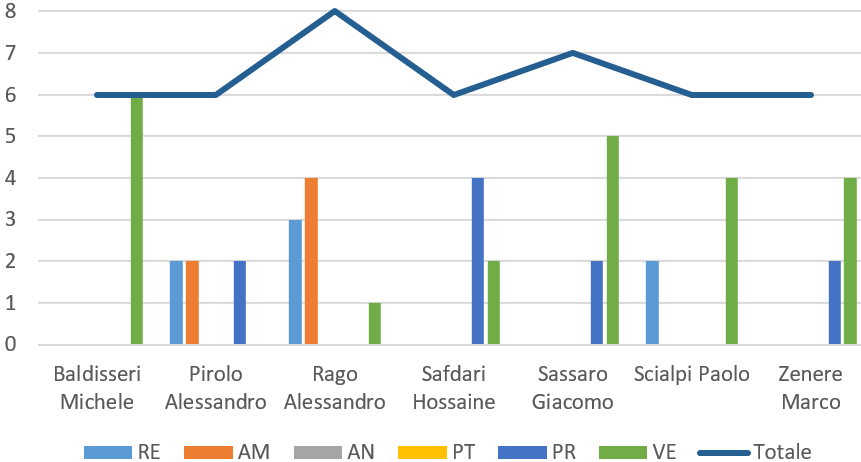
\includegraphics[width=0.95\textwidth]{Images/prev10}
	\caption{Ripartizione oraria per ciascun membro nel periodo di verifica e collaudo}
\end{figure}

%\subsubsection{Riepilogo}
%
%\begin{minipage}[b]{0.65\linewidth}
%\begin{small}
%{
%\setlength\arrayrulewidth{1pt}
%\begin{longtable}{ c | c c c c c c | c} 
% \rowcolor{coloreRosso}
% \color{white}{\textbf{Nominativo}} &
% \color{white}{\textbf{RE}} &
% \color{white}{\textbf{AM}} &
% \color{white}{\textbf{AN}} &
% \color{white}{\textbf{PT}} &
% \color{white}{\textbf{PR}} &
% \color{white}{\textbf{VE}} &
% \color{white}{\textbf{Tot.}} \\
% 	
% \BM{} & - & 5 & - & - & 4 & 11 & 20 \\ 
% \SG{} & - & - & - & - & 9 & 11 & 20 \\ 
% \SH{} & - & 3 & - & 5 & 7 & 5 & 20 \\ 
% \PA{} & 6 & 4 & - & 6 & 4 & - & 20 \\ 
% \SP{} & 4 & - & - & 4 & - & 12 & 20 \\ 
% \RA{} & 10 & 4 & - & - & - & 6 & 20 \\ 
% \ZM{} & - & 4 & - & - & 6 & 10 & 20 \\
% 
% \rowcolor{coloreRosso}
% 	\color{white}{\textbf{Totale ore ruolo}} &
% 	\color{white}{\textbf{20}} &
% 	\color{white}{\textbf{20}} &
% 	\color{white}{\textbf{-}} &
% 	\color{white}{\textbf{15}} &
% 	\color{white}{\textbf{30}} &
% 	\color{white}{\textbf{55}} &
% 	\color{white}{\textbf{140}} \\
% 	\rowcolor{white}
% 	\captionsetup{width=.9\textwidth}
% 	\caption{Distribuzione delle ore nel periodo di validazione e collaudo}
%\end{longtable}
%}
%\end{small}
%\end{minipage}
%\begin{minipage}[b]{.3\linewidth}
%\begin{small}
%{
%\setlength\arrayrulewidth{1pt}
%\begin{longtable}{ c | c | c} 
% 	\rowcolor{coloreRosso}
% 	\color{white}{\textbf{Ruolo}} &
% 	\color{white}{\textbf{Ore}} &
% 	\color{white}{\textbf{Costo €}} \\
% 	
% 	Responsabile & 20 & 600\\
% 	Amministratore & 20 & 400\\
% 	Analista & - & -\\
% 	Progettista & 15 & 330\\
% 	Programmatore & 30 & 450\\
% 	Verificatore & 55 & 825\\
% 	
% 	\rowcolor{coloreRosso}
% 	\color{white}{\textbf{Totale}} &
% 	\color{white}{\textbf{350}} &
% 	\color{white}{\textbf{2605 €}}\\
% 	\rowcolor{white}
% 	\caption{Costi per ruolo nel periodo di validazione e collaudo}
%\end{longtable}
%}
%\end{small}
%\end{minipage}
%
%I seguenti grafici riassumo i dati ottenuti.
%
%\begin{figure}[!htb]
%   \begin{minipage}{0.6\textwidth}
%     \centering
%     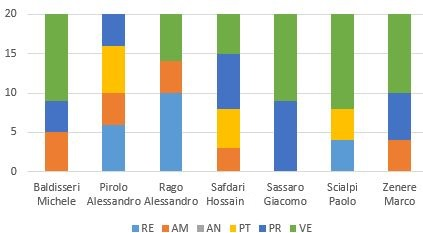
\includegraphics{Images/PO-Verifica}
%     \caption{Ripartizione oraria per ciascun membro nella fase di validazione e collaudo}
%   \end{minipage}\hspace{0.1\textwidth}
%   \begin{minipage}{0.3\textwidth}
%     \centering
%     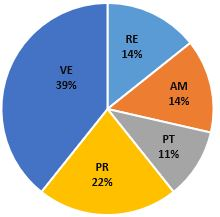
\includegraphics[width=.9\textwidth]{Images/PE-Verifica}
%     \captionsetup{width=1\textwidth}
%     \caption{Ripartizione ore totali nella fase di validazione e collaudo}
%   \end{minipage}
%\end{figure}
\subsection{Riepilogo complessivo}
\subsubsection{Ore totali}
Di seguito vengono riportate le tabelle delle ore totali utilizzate per il progetto con i relativi costi; sono considerate sia quelle d'investimento che quelle rendicontate.

\begin{minipage}[b]{0.65\linewidth}
\begin{small}
{
\setlength\arrayrulewidth{1pt}
\begin{longtable}{ c | c c c c c c | c} 
 \rowcolor{coloreRosso}
 \color{white}{\textbf{Nominativo}} &
 \color{white}{\textbf{RE}} &
 \color{white}{\textbf{AM}} &
 \color{white}{\textbf{AN}} &
 \color{white}{\textbf{PT}} &
 \color{white}{\textbf{PR}} &
 \color{white}{\textbf{VE}} &
 \color{white}{\textbf{Tot.}} \\
 	
 \BM{} & 14 & 19 & 19 & 20 & 28 & 32 & 132 \\ 
 \SG{} & 11 & 15 & 18 & 22 & 34 & 32 & 132 \\ 
 \SH{} & 6 & 13 & 22 & 22 & 36 & 33 & 132 \\ 
 \PA{} & 12 & 22 & 7 & 23 & 30 & 38 & 132 \\ 
 \SP{} & 8 & 17 & 22 & 21 & 27 & 37 & 132 \\ 
 \RA{} & 14 & 16 & 15 & 23 & 27 & 37 & 132 \\ 
 \ZM{} & 12 & 20 & 18 & 19 & 29 & 34 & 132 \\
 
 	\rowcolor{coloreRosso}
 	\color{white}{\textbf{Ore totali/ruolo}} &
 	\color{white}{\textbf{77}} &
 	\color{white}{\textbf{122}} &
 	\color{white}{\textbf{121}} &
 	\color{white}{\textbf{150}} &
 	\color{white}{\textbf{211}} &
 	\color{white}{\textbf{243}} &
 	\color{white}{\textbf{924}} \\
 	\rowcolor{white}
 	\captionsetup{width=.9\textwidth}
 	\caption{Distribuzione delle ore totali d'investimento e rendicontate}
\end{longtable}
}
\end{small}
\end{minipage}
\begin{minipage}[b]{.3\linewidth}
\begin{small}
{
\setlength\arrayrulewidth{1pt}
\begin{longtable}{ c | c | c} 
 	\rowcolor{coloreRosso}
 	\color{white}{\textbf{Ruolo}} &
 	\color{white}{\textbf{Ore}} &
 	\color{white}{\textbf{Costo €}} \\
 	
 	Responsabile & 77 & 2310\\
 	Amministratore & 122 & 2440\\
 	Analista & 121 & 3025\\
 	Progettista & 150 & 3300\\
 	Programmatore & 211 & 3165\\
 	Verificatore & 243 & 3645\\
 	
 	\rowcolor{coloreRosso}
 	\color{white}{\textbf{Totale}} &
 	\color{white}{\textbf{924}} &
 	\color{white}{\textbf{17885 €}}\\
 	\rowcolor{white}
 	\caption{Prospetto dei costi delle ore totali di investimento e rendicontate}
\end{longtable}
}
\end{small}
\end{minipage}

I seguenti grafici riassumo i dati ottenuti.

\begin{figure}[!htb]
   \begin{minipage}{0.6\textwidth}
     \centering
     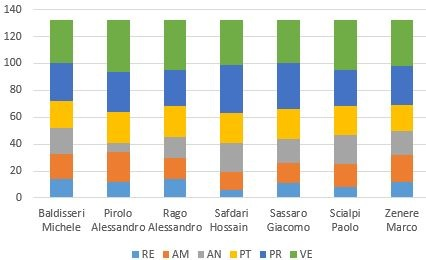
\includegraphics{Images/PO-OreTotali}
     \caption{Ripartizione oraria totale per ciascun membro}
   \end{minipage}\hspace{0.1\textwidth}
   \begin{minipage}{0.3\textwidth}
     \centering
     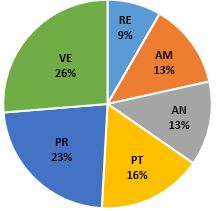
\includegraphics[width=.9\textwidth]{Images/PE-OreTotali}
     \captionsetup{width=.9\textwidth}
     \caption{Ripartizione ore totali}
   \end{minipage}
\end{figure}

\subsubsection{Ore rendicontate}
Di seguito vengono riportate le tabelle delle ore totali \textbf{rendicontate}, ovvero quelle a carico del committente.

\begin{minipage}[b]{0.65\linewidth}
\begin{small}
{
\setlength\arrayrulewidth{1pt}
\begin{longtable}{ c | c c c c c c | c} 
 \rowcolor{coloreRosso}
 \color{white}{\textbf{Nominativo}} &
 \color{white}{\textbf{RE}} &
 \color{white}{\textbf{AM}} &
 \color{white}{\textbf{AN}} &
 \color{white}{\textbf{PT}} &
 \color{white}{\textbf{PR}} &
 \color{white}{\textbf{VE}} &
 \color{white}{\textbf{Tot.}} \\
 	
 \BM{} & - & 19 & 7 & 20 & 28 & 28 & 102 \\ 
 \SG{} & - & 15 & 5 & 22 & 34 & 26 & 102 \\ 
 \SH{} & 6 & 6 & 5 & 22 & 36 & 27 & 102 \\ 
 \PA{} & 12 & 8 & 5 & 23 & 30 & 24 & 102 \\ 
 \SP{} & 8 & 17 & - & 21 & 27 & 29 & 102 \\ 
 \RA{} & 14 & 4 & 11 & 23 & 27 & 23 & 102 \\ 
 \ZM{} & 12 & 8 & 10 & 19 & 29 & 24 & 102 \\
 
 	\rowcolor{coloreRosso}
 	\color{white}{\textbf{Ore totali/ruolo}} &
 	\color{white}{\textbf{52}} &
 	\color{white}{\textbf{77}} &
 	\color{white}{\textbf{43}} &
 	\color{white}{\textbf{150}} &
 	\color{white}{\textbf{211}} &
 	\color{white}{\textbf{181}} &
 	\color{white}{\textbf{714}} \\
 	\rowcolor{white}
 	\captionsetup{width=.9\textwidth}
 	\caption{Distribuzione delle ore totali rendicontate}
\end{longtable}
}
\end{small}
\end{minipage}
\begin{minipage}[b]{.3\linewidth}
\begin{small}
{
\setlength\arrayrulewidth{1pt}
\begin{longtable}{ c | c | c} 
 	\rowcolor{coloreRosso}
 	\color{white}{\textbf{Ruolo}} &
 	\color{white}{\textbf{Ore}} &
 	\color{white}{\textbf{Costo €}} \\
 	
 	Responsabile & 52 & 1560\\
 	Amministratore & 77 & 1540\\
 	Analista & 43 & 1075\\
 	Progettista & 150 & 3300\\
 	Programmatore & 211 & 3165\\
 	Verificatore & 181 & 2715\\
 	
 	\rowcolor{coloreRosso}
 	\color{white}{\textbf{Totale}} &
 	\color{white}{\textbf{714}} &
 	\color{white}{\textbf{13355 €}}\\
 	\rowcolor{white}
 	\caption{Prospetto dei costi delle ore totali rendicontate}
\end{longtable}
}
\end{small}
\end{minipage}

I seguenti grafici riassumo i dati ottenuti.

\begin{figure}[!htb]
   \begin{minipage}{0.6\textwidth}
     \centering
     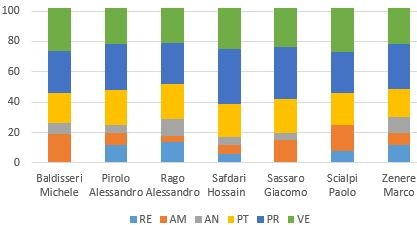
\includegraphics{Images/PO-OreRendicontate}
     \caption{Ripartizione delle ore rendicontate per ciascun membro}
   \end{minipage}\hspace{0.1\textwidth}
   \begin{minipage}{0.3\textwidth}
     \centering
     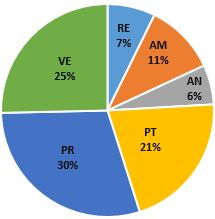
\includegraphics[width=.9\textwidth]{Images/PE-OreRendicontate}
     \captionsetup{width=.9\textwidth}
     \caption{Ripartizione ore rendicontate}
   \end{minipage}
\end{figure}


\newpage
\section{Consuntivo di periodo}

%Di seguito vengono indicate le spese effettivamente sostenute per ciascun periodo.

\subsection{Analisi dei requisiti}

Le ore di lavoro accumulate durante questa fase non sono rendicontate e vengono considerate come investimento. Pertanto la spesa non sarà a carico del proponente.

{
\setlength\arrayrulewidth{1pt}
\begin{longtable}{ C{4cm} C{3cm} C{3.5cm}} 
 	\rowcolor{coloreRosso}
 	\color{white}{\textbf{Ruolo}} &
 	\color{white}{\textbf{Ore}} &
 	\color{white}{\textbf{Costo €}} \\
 	
 	Responsabile & 25 \color{coloreRosso}{\textbf{(+5)}} & 900 \color{coloreRosso}{\textbf{(+150 €)}}\\
 	Amministratore & 45 & 900\\
 	Analista & 78 \color{coloreRosso}{\textbf{(+9)}} & 2175 \color{coloreRosso}{\textbf{(+225 €)}}\\
 	Progettista & - & -\\
 	Programmatore & - & -\\
 	Verificatore & 62 & 930\\
 	
	\hline 	
 	
 	\textbf{Totale preventivo} &
	210 &
 	4530 € \\		
 	
 	\textbf{Totale consuntivo} &
	224 &
 	4905 € \\	
 	
 	\textbf{Differenza} &
	+14 &
 	+375 € \\	
 	
 	\rowcolor{white}
 	\caption{Consuntivo del periodo di analisi dei requisiti}
\end{longtable}
}

\subsubsection{Ragione degli scostamenti}
Come si può notare dalla tabella, durante questa fase sono state richieste più ore rispetto a quelle preventivate.
\begin{itemize}
\item \textbf{Responsabile}: come riportato nella \S B, a causa dell'inesperienza, la seguente figura ha riscontrato problemi nella suddivisione del carico del lavoro, richiedendo un'analisi più minuziosa e diversi cambiamenti durante questo periodo;
\item \textbf{Analista}: come riportato nella \S B, durante la fase di analisi sono sorti diversi dubbi che hanno richiesto sia uno studio più approfondito, sia una comunicazione diretta con il proponente.
\end{itemize}

\subsubsection{Considerazioni rispetto al preventivo}
Nonostante la variazione del bilancio, non è necessario adottare alcuna contromisura poiché le ore di lavoro non sono rendicontate. Tuttavia il gruppo s'impegna ad evitare in futuro situazioni che potrebbero causare nuove variazioni al monte ore preventivato.

\subsection{Progettazione della technology baseline}
Il team si è impegnato ad apportare le modifiche segnalate alla precedente revisione sulla maggior parte dei documenti, oltre ad integrarli e ad individuare le tecnologie necessarie allo sviluppo del prodotto.

{
\setlength\arrayrulewidth{1pt}
\begin{longtable}{ C{4cm} C{3cm} C{3.5cm}} 
 	\rowcolor{coloreRosso}
 	\color{white}{\textbf{Ruolo}} &
 	\color{white}{\textbf{Ore}} &
 	\color{white}{\textbf{Costo €}} \\
 	
 	Responsabile & 4 & 120 €\\
 	Amministratore & 8 & 160 €\\
 	Analista & 19 \color{coloreRosso}{\textbf{(-2)}} & 475 € \color{coloreRosso}{\textbf{(-50 €)}}\\
 	Progettista & 24 & 528 €\\
 	Programmatore & 4 \color{coloreRosso}{\textbf{(+4)}} & 60 € \color{coloreRosso}{\textbf{(+60 €)}}\\
 	Verificatore & 27 \color{coloreRosso}{\textbf{(-5)}} & 405 € \color{coloreRosso}{\textbf{(-75 €)}}\\
 	
	\hline 	
 	
 	\textbf{Totale preventivo} &
	86 &
 	1748 € \\		
 	
 	\textbf{Totale consuntivo} &
	83 &
 	1683 € \\	
 	
 	\textbf{Differenza} &
	-3 &
 	-65 € \\	
 	
 	\rowcolor{white}
 	\caption{Consuntivo del periodo di progettazione della TB}
\end{longtable}
}

\subsubsection{Ragione degli scostamenti}
 
\begin{itemize}
\item \textbf{Analista (-2 ore)}: grazie alla buona base prodotta nella fase precedente, sono servite meno ore di quelle preventivate in quanto, l'\textit{Analisi dei Requisiti}, è stata per lo più integrata;

\item \textbf{Programmatore (+4 ore)}: la seguente figura ha occupato più tempo di quello che si era previsto per testare le tecnologie individuate;

\item \textbf{Verificatore (-5 ore)}: poiché il lavoro degli analisti e degli amministratori è stato svolto con precisione e in breve tempo, anche il lavoro dei verificatori è stato più veloce del previsto.
\end{itemize}

\subsubsection{Considerazioni rispetto al preventivo}

Il bilancio è positivo rispetto al preventivo per questo periodo. Non si ritiene comunque necessaria alcuna ripianificazione del prossimo incremento in quanto la somma risparmiata non è significativa. Inoltre, avendo raggiunto tutti gli obiettivi, l'avanzamento delle attività non ha subito rallentamenti.

\newpage

\subsection{Incremento I}
Durante questo incremento il gruppo si è occupato di terminare i lavori in fase di conclusione e ad iniziare lo sviluppo del \glo{PoC}. Tutti gli obiettivi sono stati raggiunti, rispettando le milestone interne.
{
\setlength\arrayrulewidth{1pt}
\begin{longtable}{ C{4cm} C{3cm} C{3.5cm}} 
 	\rowcolor{coloreRosso}
 	\color{white}{\textbf{Ruolo}} &
 	\color{white}{\textbf{Ore}} &
 	\color{white}{\textbf{Costo €}} \\
 	
 	Responsabile & 2 \color{coloreRosso}{\textbf{(+1)}} & 60 € \color{coloreRosso}{\textbf{(+30 €)}}\\
 	Amministratore & 12 & 240 €\\
 	Analista & 20 & 500 € \\
 	Progettista & 24 \color{coloreRosso}{\textbf{(-2)}} & 528 € \color{coloreRosso}{\textbf{(-44 €)}}\\
 	Programmatore & 14 & 210 € \\
 	Verificatore & 9  & 135 €\\
 	
	\hline 	
 	
 	\textbf{Totale preventivo} &
	81 &
 	1673 € \\		
 	
 	\textbf{Totale consuntivo} &
	80 &
 	1659 € \\	
 	
 	\textbf{Differenza} &
	-1 &
 	-14 € \\	
 	
 	\rowcolor{white}
 	\caption{Consuntivo dell'incremento I}
\end{longtable}
}

\subsubsection{Ragione degli scostamenti}

\begin{itemize}
\item \textbf{Responsabile (+1 ora)}: il tempo richiesto per ultimare il \textit{Piano di Progetto} è stato leggermente più del dovuto. Parte del rallentamento è stato causato anche dal complicato coordinamento delle attività da svolgere in questa fase;

\item \textbf{Progettista (-2 ore)}: la progettazione necessaria all'incremento, grazie all'esperienza maturata in precedenza, ha richiesto meno ore del previsto.

\end{itemize}

\subsubsection{Considerazioni rispetto al preventivo}

In base al risultato ottenuto, si è potuto constatare che le ore pianificate per questo incremento sono risultate nel complesso corrette. Nonostante le piccole variazioni, il bilancio risulta essere positivo rispetto al preventivo per questo periodo. Non si ritiene comunque necessaria alcuna ripianificazione in quanto la somma risparmiata non è significativa. Inoltre, visto il raggiungimento di tutti gli obiettivi, le attività future, per il momento, non subiranno modifiche.

\newpage

\subsection{Incremento II}
Durante questo incremento il team si è concentrato ad ultimare il \glo{PoC}, ovvero nell'implementazione del primo grafico che il prodotto dovrà offrire. Tutti gli obiettivi sono stati raggiunti.%, rispettando le milestone interne.

{
\setlength\arrayrulewidth{1pt}
\begin{longtable}{ C{4cm} C{3cm} C{3.5cm}} 
 	\rowcolor{coloreRosso}
 	\color{white}{\textbf{Ruolo}} &
 	\color{white}{\textbf{Ore}} &
 	\color{white}{\textbf{Costo €}} \\
 	
 	Responsabile & 6 & 180 € \\
 	Amministratore & 10 & 200 €\\
 	Analista & 4 \color{coloreRosso}{\textbf{(-1)}} & 100 € \color{coloreRosso}{\textbf{(-25 €)}}\\
 	Progettista & 12 & 264 € \\
 	Programmatore & 16 \color{coloreRosso}{\textbf{(+2)}} & 240 € \color{coloreRosso}{\textbf{(+30 €)}}\\
 	Verificatore & 9 \color{coloreRosso}{\textbf{(+4)}} & 135 \color{coloreRosso}{\textbf{(+60)}}€\\
 	
	\hline 	
 	
 	\textbf{Totale preventivo} &
	57 &
 	1119 € \\		
 	
 	\textbf{Totale consuntivo} &
	62 &
 	1194 € \\	
 	
 	\textbf{Differenza} &
	+5 &
 	+75 € \\	
 	
 	\rowcolor{white}
 	\caption{Consuntivo dell'incremento II}
\end{longtable}
}

\subsubsection{Ragione degli scostamenti}

\begin{itemize}
\item \textbf{Analista (-1 ore)}: grazie ad una comunicazione costante con il proponente, gli analisti hanno individuato rapidamente degli algoritmi di calcolo della distanza tra i dati;

\item \textbf{Programmatore (+2 ore)}: sono state riscontrate alcune difficoltà nell'implementare la visualizzazione \glo{\textit{Scatter Plot Matrix}} in modo dinamico, ovvero nella creazione automatica dei singoli \glo{\textit{Scatter Plot}} in base al set di dati caricato;

\item \textbf{Verificatore (+4 ore)}: quasi tutte le ore che non erano state utilizzate nel primo incremento sono state impiegate per garantire una maggiore qualità dei documenti.
\end{itemize}
\subsubsection{Considerazioni rispetto al preventivo}

Sulla base degli obiettivi prefissati, il consumo di risorse durante questo incremento è stato notevole e il bilancio risulta negativo rispetto al preventivo; tuttavia non si ritiene necessaria alcuna ripianificazione in quanto sono state utilizzate le ore risparmiate negli incrementi precedenti, mantenendo un bilancio in positivo rispetto al totale. Visto il raggiungimento di tutti gli obiettivi prefissati non sono previsti interventi sulla pianificazione del prossimo incremento.

\newpage

\subsection{Incremento III}
Durante questo incremento il team si è concentrato nel consolidare il design pattern architetturale scelto e ad implementare una componente per la riduzione dimensionale. Tutti gli obiettivi pianificati dal team sono stati raggiunti.
{
\setlength\arrayrulewidth{1pt}
\begin{longtable}{ C{4cm} C{3cm} C{3.5cm}} 
 	\rowcolor{coloreRosso}
 	\color{white}{\textbf{Ruolo}} &
 	\color{white}{\textbf{Ore}} &
 	\color{white}{\textbf{Costo €}} \\
 	
 	Responsabile & 4 & 120 € \\
 	Amministratore & 5 & 100 €\\
 	Analista & -& - \\
 	Progettista & 13 \color{coloreRosso}{\textbf{(+2)}} & 286 € \color{coloreRosso}{\textbf{(+44 €)}}\\
 	Programmatore & 23 & 345 € \\
 	Verificatore & 20 \color{coloreRosso}{\textbf{(-5)}} & 300 € \color{coloreRosso}{\textbf{(-75 €)}}\\
 	
	\hline 	
 	
 	\textbf{Totale preventivo} &
	65 &
 	1151 € \\		
 	
 	\textbf{Totale consuntivo} &
	62 &
 	1120 € \\	
 	
 	\textbf{Differenza} &
	-3 &
 	-31 € \\	
 	
 	\rowcolor{white}
 	\caption{Consuntivo dell'incremento III}
\end{longtable}
}

\subsubsection{Ragione degli scostamenti}


\begin{itemize}
\item \textbf{Progettista (+2 ore)}: sono state riscontrate varie difficoltà nel capire come suddividere la logica delle componenti grafiche e nell'integrare \glo{Mobx} nell'architettura;
\item \textbf{Verificatore (-5 ore)}: la quantità di codice prodotto non è stata significativa, di conseguenza non sono stati necessari molti interventi da parte della seguente figura.
\end{itemize}

\subsubsection{Considerazioni rispetto al preventivo}

Nonostante il lieve aumento nel consumo delle risorse da parte dei progettisti, il non utilizzo di tutte le ore da verificatore ha portato ad un esito positivo del bilancio. Tuttavia non si ritiene necessaria alcuna ripianificazione poiché la somma non è significativa e sarà certamente recuperata negli incrementi successivi.\\ 
Avendo raggiunto tutti gli obiettivi l'avanzamento delle attività non ha subito rallentamenti.

\newpage

\subsection{Incremento IV}
Durante questo incremento il team si è concentrato nell'ultimare la riduzione dimensionale tramite calcolo della distanza e nella realizzazione del grafico \glo{Adjacency Matrix}. Tutti gli obiettivi prefissati dal gruppo sono stati raggiunti.
{
\setlength\arrayrulewidth{1pt}
\begin{longtable}{ C{4cm} C{3cm} C{3.5cm}} 
 	\rowcolor{coloreRosso}
 	\color{white}{\textbf{Ruolo}} &
 	\color{white}{\textbf{Ore}} &
 	\color{white}{\textbf{Costo €}} \\
 	
 	Responsabile & 4 & 120 € \\
 	Amministratore & 5 & 100 €\\
 	Analista & - & - \\
 	Progettista & 23 & 506 € \\
 	Programmatore & 28 \color{coloreRosso}{\textbf{(+3)}} & 420 € \color{coloreRosso}{\textbf{(+45 €)}}\\
 	Verificatore & 14 & 210 €\\
 	
	\hline 	
 	
 	\textbf{Totale preventivo} &
	74 &
 	1356 € \\		
 	
 	\textbf{Totale consuntivo} &
	77 &
 	1401 € \\	
 	
 	\textbf{Differenza} &
	+3 &
 	+45 € \\	
 	
 	\rowcolor{white}
 	\caption{Consuntivo dell'incremento IV}
\end{longtable}
}

\subsubsection{Ragione degli scostamenti}

\begin{itemize}
\item \textbf{Programmatore (+3 ore)}: il calcolo delle distanze e l'implementazione dell'ordinamento della matrice nella nuova versione della libreria \glo{D3.js} hanno causato alcuni rallentamenti. 
\end{itemize}

\subsubsection{Considerazioni rispetto al preventivo}

In base al risultato ottenuto, si è potuto constatare che le ore pianificate per questo incremento sono risultate nel complesso corrette. Tuttavia il lieve aumento nel consumo delle risorse ha causato un esito negativo sul bilancio rispetto al preventivo.\\
Non si ritiene necessaria alcuna ripianificazione poiché la somma non è significativa ed è in parte bilanciata da quanto risparmiato nell’incremento precedente. Inoltre, avendo raggiunto tutti gli obiettivi l'avanzamento delle attività non ha subito rallentamenti. Vista la portata limitata del prossimo incremento, il team conta di bilanciare nelle prossime settimane l'eccesso di risorse consumate.

\newpage

\subsection{Incremento V}
Durante questo incremento il team si è concentrato principalmente nell'implementazione del grafico \glo{Force Field}.
{
\setlength\arrayrulewidth{1pt}
\begin{longtable}{ C{4cm} C{3cm} C{3.5cm}} 
 	\rowcolor{coloreRosso}
 	\color{white}{\textbf{Ruolo}} &
 	\color{white}{\textbf{Ore}} &
 	\color{white}{\textbf{Costo €}} \\
 	
 	Responsabile & 3 & 90 € \\
 	Amministratore & 6 & 120 €\\
 	Analista & - & - \\
 	Progettista & 20 \color{coloreRosso}{\textbf{(-3)}} & 440 € \color{coloreRosso}{\textbf{(-66 €)}}\\
 	Programmatore & 27 \color{coloreRosso}{\textbf{(-3)}} & 405 € \color{coloreRosso}{\textbf{(-45 €)}}\\
 	Verificatore & 12 & 180 €\\
 	
	\hline 	
 	
 	\textbf{Totale preventivo} &
	68 &
 	1235 € \\		
 	
 	\textbf{Totale consuntivo} &
	62 &
 	1124 € \\	
 	
 	\textbf{Differenza} &
	-6 &
 	-111 € \\	
 	
 	\rowcolor{white}
 	\caption{Consuntivo dell'incremento V}
\end{longtable}
}

\subsubsection{Ragione degli scostamenti}

\begin{itemize}
\item \textbf{Progettista (-3 ore)}: vista la similitudine a livello logico ed implementativo del grafico rispetto al precedente introdotto, non sono state utilizzate tutte le ore pianificate;
\item \textbf{Programmatore (-3 ore)}: grazie all'esperienza maturata nell'utilizzo della libreria D3.js, anche per la seguente figura non sono state consumate tutte le ore pianificate.
\end{itemize}

\subsubsection{Considerazioni rispetto al preventivo}

Il non utilizzo di tutte le ore pianificate ha portato ad un esito positivo del bilancio rispetto al preventivo di questo incremento. Tuttavia non si ritiene necessaria alcuna ripianificazione poiché la somma va a bilanciare in parte le spese eccessive sostenute negli incrementi precedenti. Inoltre parte della differenza sarà sicuramente recuperata nel prossimo incremento, vista la notevole portata. 

Degli obiettivi pianificati non è stato portato al grado di avanzamento desiderato la stesura dei manuali. Questo compito avrà massima priorità nel prossimo incremento, eventualmente assegnando più ore di lavoro. Ciò nonostante la codifica del prodotto software è a un buon punto e, grazie anche alla padronanza acquisita nell'utilizzo della libreria D3.js, il team prevede di riuscire a contenere i costi e a rispettare il preventivo nel prossimo incremento.

\newpage

\subsection{Incremento VI}
Durante questo incremento il team si è concentrato ad implementare i grafici \glo{Proiezione Lineare Multi Asse} e \glo{Heat Map}.

{
\setlength\arrayrulewidth{1pt}
\begin{longtable}{ C{4cm} C{3cm} C{3.5cm}} 
 	\rowcolor{coloreRosso}
 	\color{white}{\textbf{Ruolo}} &
 	\color{white}{\textbf{Ore}} &
 	\color{white}{\textbf{Costo €}} \\
 	
 	Responsabile & 3 \color{coloreRosso}{\textbf{(+1)}} & 60 € \color{coloreRosso}{\textbf{(+30 €)}}\\
 	Amministratore & 5 & 100 €\\
 	Analista & - & - \\
 	Progettista & 11 & 242 € \\
 	Programmatore & 33 \color{coloreRosso}{\textbf{(-2)}} & 495 € \color{coloreRosso}{\textbf{(-30 €)}}\\
 	Verificatore & 16 & 240 €\\
 	
	\hline 	
 	
 	\textbf{Totale preventivo} &
	68 &
 	1167 € \\		
 	
 	\textbf{Totale consuntivo} &
	67 &
 	1167 € \\	
 	
 	\textbf{Differenza} &
	-1 &
 	- € \\	
 	
 	\rowcolor{white}
 	\caption{Consuntivo dell'incremento VI}
\end{longtable}
}

\subsubsection{Ragione degli scostamenti}

\begin{itemize}
\item \textbf{Responsabile (+1 ora)}: vista la decisione, in seguito al colloquio con il proponente, nell'aggiunta di un nuovo grafico la seguente figura ha avuto bisogno di più tempo del previsto per assegnare i compiti da svolgere in modo ottimale;
\item \textbf{Programmatore (-2 ore)}: l'implementazione della visualizzazione \glo{PLMA}, che il gruppo riteneva complessa, è stata svolta utilizzando meno ore del previsto. 
\end{itemize}

\subsubsection{Considerazioni rispetto al preventivo}
Tutti gli obiettivi sono stati raggiunti con successo. Il bilancio dell'incremento risulta comunque essere in pari, nonostante il consumo delle risorse non sia stato pienamente rispettato.

L'andamento delle attività di progetto non ha subito rallentamenti e il gruppo è riuscito ad implementare quanto era stato previsto per l'incremento IX. Per questo motivo si è deciso di attuare una ripianificazione per i prossimi incrementi. Le ore recuperate verranno utilizzate in parte durante la fase di verifica e collaudo, mentre le rimanenti saranno usate nel prossimo incremento. Al termine dell'incremento VII infatti, il gruppo dovrà sostenere la verifica sulla \textit{product baseline} e, in caso di raffinamenti, potrebbero essere necessarie delle ore aggiuntive rispetto a quelle pianificate in precedenza. 

\subsection{Incremento VII}
Durante questo incremento il gruppo si è concentrato principalmente ad implementare la connessione con il database per il recupero dei dati.
{
\setlength\arrayrulewidth{1pt}
\begin{longtable}{ C{4cm} C{3cm} C{3.5cm}} 
 	\rowcolor{coloreRosso}
 	\color{white}{\textbf{Ruolo}} &
 	\color{white}{\textbf{Ore}} &
 	\color{white}{\textbf{Costo €}} \\
 	
 	Responsabile & 8 & 240 € \\
 	Amministratore & 10 & 200 €\\
 	Analista & - & - \\
 	Progettista & 20 & 440 € \\
 	Programmatore & 40 \color{coloreRosso}{\textbf{(-6)}} & 600 € \color{coloreRosso}{\textbf{(-90 €)}}\\
 	Verificatore & 19 \color{coloreRosso}{\textbf{(+6)}} & 285 € \color{coloreRosso}{\textbf{(+90 €)}}\\
 	
	\hline 	
 	
 	\textbf{Totale preventivo} &
	97 &
 	1765 € \\		
 	
 	\textbf{Totale consuntivo} &
	97 &
 	1765 € \\	
 	
 	\textbf{Differenza} &
	- &
 	- € \\	
 	
 	\rowcolor{white}
 	\caption{Consuntivo dell'incremento VII}
\end{longtable}
}

\subsubsection{Ragione degli scostamenti}

\begin{itemize}
\item \textbf{Programmatore (-6 ore)}: poiché durante il periodo di progettazione di \textit{technology baseline} le tecnologie usate erano già state testate, la seguente figura ha occupato meno tempo del previsto; 

\item \textbf{Verificatore (+6 ore)}: i raffinamenti attuati a livello architetturale hanno richiesto un intervento maggiore da parte del verificatore.
\end{itemize}

\subsubsection{Considerazioni rispetto al preventivo}

In base al risultato ottenuto, nonostante il consumo delle risorse previsto non sia stato rispettato, il bilancio rispetto al preventivo di questo incremento risulta essere in pari. Rispetto al bilancio complessivo, questa fase termina in positivo, seppur di una quantità poco significativa. \\
Il gruppo non è completamente soddisfatto della parte di test implementata fino a questo momento. Questa attività avrà una priorità maggiore nelle prossime settimane, eventualmente assegnando più ore di lavoro. Ciò nonostante il team ha raggiunto dei risultati appaganti e prevede di riuscire a contenere i costi e a rispettare i preventivi dei prossimi incrementi, oltre alle scadenze dettate dalla nuova pianificazione.

\newpage

\subsection{Riepilogo}

Di seguito viene riportata la tabella con il riepilogo dei preventivi e consuntivi riferiti agli incrementi sostenuti fino a questo momento, con relativo impatto sull'importo complessivo.
{
\setlength\arrayrulewidth{1pt}
\begin{longtable}{ C{1.5cm} | C{3.4cm} | C{3.4cm} | C{3cm} | C{3.4cm}} 
   \rowcolor{coloreRosso}
   \color{white}{\textbf{Incr.}} &
   \color{white}{\textbf{Preventivo}} &
   \color{white}{\textbf{Consuntivo}} & 
   \color{white}{\textbf{Sostenuto}} &
   \color{white}{\textbf{Scostamento}} \\
   
   TB & 1.748,00€ , 86 ore & 1.683,00 € , 83 ore & \begin{LARGE}\redcheck \end{LARGE} & -65,00€ , -3 ore\\
   
   I & 1.673,00€ , 81 ore & 1.659,00€ , 80 ore & \begin{LARGE}\redcheck \end{LARGE} & -14,00€ , -1 ora\\
   
   II & 1.119,00€ , 57 ore & 1.194,00€ , 62 ore & \begin{LARGE}\redcheck \end{LARGE} & +75,00€ , +5 ore\\
   
   III & 1.151,00€ , 65 ore & 1.120,00€ , 62 ore & \begin{LARGE}\redcheck \end{LARGE} & -31,00€ , -3 ore\\
   
   IV & 1.356,00€ , 74 ore & 1.401,00€ , 77 ore & \begin{LARGE}\redcheck \end{LARGE} & +45,00€ , +3 ore\\
   
   V & 1.235,00€ , 68 ore & 1.124,00€ , 62 ore & \begin{LARGE}\redcheck \end{LARGE} & -111,00€ , -6 ore\\
   
   VI & 1.167,00€ , 68 ore & 1.167,00€ , 67 ore & \begin{LARGE}\redcheck \end{LARGE} & 0,00€ , -1 ora\\
   
   VII & 1.765,00€ , 97 ore & 1.765,00€ , 97 ore & \begin{LARGE}\redcheck \end{LARGE} & 0,00 € , 0 ore\\
   
   \rowcolor{coloreRossoChiaro}
   \color{white}\textbf{Totale} & \color{white}11.214,00€ , 596 ore & \color{white}11.113,00€ , 590 ore & & \color{white}-101,00€ , -6 ore\\
   
   VIII & 1.331,00€ , 73 ore &  &  & \\
   
   V/C & 810,00€ , 45 ore & &  & \\
   
   \textbf{Totale} & \textbf{13.355,00€} \newline \textbf{714 ore} & \textbf{13.254,00€} \newline \textbf{708 ore} &  &\\
   
   \rowcolor{white}
   \caption{Riepilogo preventivo e consuntivo}
\end{longtable}
}

\newpage

\appendix
\section{Organigramma}
\subsection{Redazione}
\begin{longtable}{ c  c  c} 
 	\rowcolor{coloreRosso}
 	\color{white}{\textbf{Nominativo}} &
 	\color{white}{\textbf{Data}} &
 	\color{white}{\textbf{Firma}} \\
 	
 	\BM{} & 07-01-2021 & 
\includegraphics[scale=0.3]{Images/firmaMB.png} \\
 	\SG{} & 07-01-2021 & 
\includegraphics[scale=0.15]{Images/firmaSG.png} \\
 	\PA{} & 07-01-2021 & 
\includegraphics[scale=0.08]{Images/firmaPA.png} \\
 	\rowcolor{white}\caption{Data e firma di redazione dei redattori}
\end{longtable}

\subsection{Approvazione}
\begin{longtable}{ c  c  c} 
 	\rowcolor{coloreRosso}
 	\color{white}{\textbf{Nominativo}} &
 	\color{white}{\textbf{Data}} &
 	\color{white}{\textbf{Firma}} \\
 	
 	\SG{} & 09-01-2021 & 
\includegraphics[scale=0.15]{Images/firmaSG.png} \\
 	Prof. Vardanega Tullio &  &  \\
 	Prof. Cardin Riccardo &  &  \\
 	\rowcolor{white}\caption{Data e firma di approvazione degli approvatori}
\end{longtable}

\newpage

\subsection{Accettazione dei componenti}
\begin{longtable}{ c  c  c} 
 	\rowcolor{coloreRosso}
 	\color{white}{\textbf{Nominativo}} &
 	\color{white}{\textbf{Data}} &
 	\color{white}{\textbf{Firma}} \\
 	
 	\BM{} & 07-01-2021 & 
\includegraphics[scale=0.3]{Images/firmaMB.png} \\
 	\SG{} & 07-01-2021 & 
\includegraphics[scale=0.15]{Images/firmaSG.png} \\
 	\SH{} & 07-01-2021 & 
\includegraphics[scale=0.08]{Images/firmaSH.png} \\
 	\ZM{} & 07-01-2021 & 
\includegraphics[scale=0.3]{Images/firmaZM.png} \\
 	\SP{} & 07-01-2021 & 
\includegraphics[scale=0.18]{Images/firmaSP.png} \\
 	\RA{} & 07-01-2021 & 
\includegraphics[scale=0.25]{Images/firmaRA.png} \\
 	\PA{} & 07-01-2021 & 
\includegraphics[scale=0.08]{Images/firmaPA.png} \\
	
	\rowcolor{white}\caption{Data e firma di accettazione dei componenti}
\end{longtable}
\subsection{Componenti}
\begin{longtable}{ c  c  c} 
 	\rowcolor{coloreRosso}
 	\color{white}{\textbf{Nominativo}} &
 	\color{white}{\textbf{Matricola}} &
 	\color{white}{\textbf{Contatto}} \\
 	
 	\BM{} & 1193109 & michele.baldisseri@studenti.unipd.it \\
 	\SG{} & 1187566 & giacomo.sassaro@studenti.unipd.it \\
 	\SH{} & 1102482 & hossain.safdari@studenti.unipd.it \\
 	\ZM{} & 1123576 & marco.zenere.1@studenti.unipd.it \\
 	\SP{} & 1161625 & paolo.scialpi@studenti.unipd.it \\
 	\RA{} & 1187504 & alessandro.rago.1@studenti.unipd.it \\
 	\PA{} & 1193361 & alessandro.pirolo@studenti.unipd.it \\
 	
 	\rowcolor{white}\caption{Dati dei componenti del gruppo}
\end{longtable}


\newpage
\section{Attualizzazione dei rischi}

Questa sezione riporta i rischi che si sono effettivamente verificati e come il gruppo si è dedicato alla loro risoluzione.

\begin{longtable}{C{2.5cm} C{7cm} C{7cm}} 
 	\rowcolor{coloreRosso}
 	\color{white}{\textbf{Rischio}} &
 	\color{white}{\textbf{Descrizione}} &
 	\color{white}{\textbf{Mitigazione}} \\
 	
 	RI1 & A causa della situazione di emergenza sanitaria dovuta al virus \textit{Covid-19} il gruppo ha avuto modo di collaborare solamente a distanza. & Tutti i componenti hanno comunicato il più possibile, aggiornandosi reciprocamente in modo costante sull'andamento dei lavori e su eventuali problemi riscontrati. \\
 	RI4 & Il gruppo ha riscontrato alcuni dubbi in merito alla realizzazione del prodotto finale, causando alcuni rallentamenti durante la redazione dei documenti. & Il team, in seguito a diverse discussioni, ha deciso di mettersi nuovamente in contatto con il \textit{proponente} per avere dei chiarimenti. \\
 	
 	\rowcolor{white}
 	\caption{Attualizzazione dei rischi}
\end{longtable}
\end{document}